% \documentclass[linenumbers, manuscript]{aastex631}
\documentclass{aastex631}
\newcommand{\vdag}{(v)^\dagger}
\newcommand\aastex{AAS\TeX}
\newcommand\latex{La\TeX}
\usepackage{mathtools}

\begin{document}

\title{A Trans-Neptunian Object and Solar System Object Discovery Method with Convolutional Neural Networks for Future Surveys}
\author[0000-0002-4258-2964]{Aram I}
\affiliation{University of Victoria, Department of Physics and Astronomy, Elliott Building, 3800 Finnerty Road, Victoria, British Columbia, Canada, V8P 5C2}
\author[0000-0002-4258-2964]{J. J. Kavelaars}
\affiliation{University of Victoria, Department of Physics and Astronomy, Elliott Building, 3800 Finnerty Road, Victoria, British Columbia, Canada, V8P 5C2}
\affiliation{NRC Herzberg Astronomy and Astrophysics, 5071 West Saanich Road, Victoria, British Columbia, Canada, V9E 2E7}
\affiliation{Department of Physics and Astronomy, University of British Columbia, 6224 Agricultural Road, Vancouver, BC V6T 1Z1, Canada}
\author[0000-0002-4258-2964]{Hossen Teimoorinia}
\affiliation{University of Victoria, Department of Physics and Astronomy, Elliott Building, 3800 Finnerty Road, Victoria, British Columbia, Canada, V8P 5C2}
\affiliation{NRC Herzberg Astronomy and Astrophysics, 5071 West Saanich Road, Victoria, British Columbia, Canada, V9E 2E7}
\author[0000-0002-4258-2964]{Wesley Fraser}
\affiliation{University of Victoria, Department of Physics and Astronomy, Elliott Building, 3800 Finnerty Road, Victoria, British Columbia, Canada, V8P 5C2}
\affiliation{NRC Herzberg Astronomy and Astrophysics, 5071 West Saanich Road, Victoria, British Columbia, Canada, V9E 2E7}
\author[0000-0002-4258-2964]{Edward Ashton}
\affiliation{Institute of Astronomy and Astrophysics, Academia Sinica, Taipei, Taiwan}

\begin{abstract}

% Title
We present a deep learning method of searching for Trans-Neptunian objects (TNOs) and solar system objects (SSOs) in wide-field survey imaging data.
% Method 1
Our deep learning approach is based on the detection of moving sources within 64$\times$64-pixel sub-image pairs extracted from large-format mosaic imaging data.
We trained our CNNs using artificially generated sources added to CFHT MegaCam images.
Each image pair extracted from the training images has been labeled with the presence or absence of a moving source, along with the source location and magnitude.
The labeled sub-images were fed into ImageNet algorithms to train classification models and regression models separately.
% Result 1
A trained classification model derived from the MobileNet model retrieved 91\% of sub-images with a moving source with a 90\% precision on test data sets.
A separate regression model then predicts the location of the moving source with a mean absolute error of $\pm1.5$ pixels for sources over SNR$\geq$16.5.
% (22 $\leq$ m $<$ 23)
% Method 2
With the classification-filtered sub-images and their regression-measured locations in sky coordinates, each detected source was grouped with nearby detected sources based on the assumption that SSOs will exhibit linear sky motion during the observed period. 
Any group of linear sources, tracks, having at least 11 detections was then considered a candidate detection.
% Result 2
After the candidate-making process, we achieved effective detection limit of SNR=7.2.
However, with this linear fitting approach, only a handful of SSOs were discovered.
% Method 3
We also examined an alternative scoring approach, where images were scored based on the probability values from the classification model.
% Result 3
With this approach, we achieved an effective detection limit of SNR=3.4.
Moreover, we found approximately 200 visibly bright real SSO candidates among approximately 1800 candidates.
% Discussion
We tested trained models on test sets from different sky regions and discovered that our models did not learn from the backgrounds or shapes of TNOs, but rather detected the motion of TNOs.
% Conclusion
This paper shows deep learning object detection algorithms can aid in the discovery of TNOs and SSOs, supporting future discovery pipeline development.

\end{abstract}

\keywords{Solar system(1528) --- Kuiper belt(893) --- Detection(1911) --- Neural networks(1933)}

\section{Introduction} \label{sec:intro}
Trans-Neptunian Objects (TNOs) are the population of small solar system objects with a semi-major axis of more than 30~au (Neptune) and less than about 2000~au (Oort Cloud), and solar system objects (SSOs) are all natural bodies in the solar system that are neither the Sun nor planets.
TNOs exhibit a range of physical sizes, albedos, shapes, surface colors and appear in a variety of different orbits.
Some TNOs are as large as thousands of kilometers in diameter, while the smallest known objects are of order 10~km in diameter.
Likewise, some have nearly circular and low-inclination orbits (e.g. 79360 Sila-Nunam) \citep{1997MPEC....N...08L}, while others have highly eccentric (e.g. 541132 Leleākūhonua) \citep{2019AJ....157..139S} or highly inclined orbits (e.g. 136472 Makemake) \citep{2005IAUC.8577....1B}.
By searching for and discovering a large sample of diverse TNOs we can better understand the processes of planet formation and migration at work in the solar system.  
To achieve this goal requires developing efficient algorithms and processes for the discovery of these faint, slow-moving bodies.

Wide-field image TNO surveys, such as the Dark Energy Survey \citep{2020ApJS..247...32B} and the Outer Solar System Origins Survey \citep{2016AJ....152...70B}, used dedicated TNO discovery pipelines, Developing such pipelines is a time-consuming task.
These surveys, and others, rely on detecting ``features'', or sources. 
Determining which of those features remain stationary and then determining if any of the non-static features can be grouped in a way that is consistent with the expected linear motion of a solar system body \citep[see][for a complete description of such a detection system]{2004MNRAS.347..471P}.
A key component of the feature detection process is that one first engineers what features of interest might look like (e.g. a two-dimensional Gaussian with a particular profile width) and then uses convolutional processes to search similar features within the data.
This feature detection process relies on knowledge of the image quality and often needs to be tuned for the data taken on specific nights.
Our goal was to conduct moving source detection directly from the pixel data.
Working directly from the pixel data removes the need for feature-engineering based source catalogues \citep[section 3]{2016AJ....151..158F} and may provide a more universally usable detection process.
We refer to this as feature-agnostic moving source detection.

We demonstrate, using data acquired for a TNO specific search, that our technique detects TNOs as faint as those found in the original search while providing a low false-positive rate.
Using this detection pipeline will aid in the detection of TNOs in imaging not specifically tuned to TNO dedication, such as the wide layer of Canada-France Imaging Survey \citep{2017ApJ...848..128I}, which acquired imaging with 10 or 20 minutes between visits pairs and a total exposure time of 150 or 200 seconds of exposure time per visit.

Section \ref{sect: Techniques} briefly summarizes the deep neural network (DNN) techniques we used.
Section \ref{sect: Data} describes the data preparation.
Section \ref{sect: Model Selection} compares trained DNN models, and the best classification/regression model for TNO detection was selected and implemented on our data set.
Section \ref{sect: Implementation} describes how we used trained models for precise and time-efficient image analysis.
Section \ref{sect: Data}, \ref{sect: Model Selection}, and \ref{sect: Implementation} make the method part of this paper all together.
If you are familiar with machine learning, reading section \ref{sect: Model Selection} and \ref{sect: Implementation} would be helpful to find SSOs with a similar approach.
In section \ref{sect: Results}, we search data for TNOs, and conclude that the developed method can be used for other surveys as well.

\section{Image Recognition Deep Learning Techniques}
\label{sect: Techniques}
Modern and effective image recognition neural networks are deep and convolutional. 
Deep neural networks (DNNs) have hidden layers between the input and output layers.
Those hidden layers are connected via weights that are initially random or uniform numbers and then optimized during the model training. 
(A ``model" is a program that has been trained on a set of data to recognize certain types of patterns.)
Back-propagation and stochastic gradient descent are used to change the initial weights to match the characteristics of the output layer against training labels \citep{lecun1988theoretical, bottou2012stochastic}.
The trained weights act as circuits that identify features of the image input, thus, the algorithm learns from the image what the image features are rather than having those imposed at a source detection step. 
For example, some weights could be switches that only turn on if the input image has a bright galaxy filling the background. 
The training process of DNN is the process of extracting features from the training set, and training the weights to predict the class of the image as the output layer \citep{fukushima1983neocognitron}.

\subsection{Tested Architectures}

We explored a number of network architectures to determine which might be most effective at moving source detection. Here we briefly describe each of these architectures and then report on their accuracy and determine the most effective architecture for our problem.

\label{subsect: Tested Architectures}
\subsubsection{Fully-connected Neural Networks}
\label{subsubsect:FCNNs}
A fully-connected neural network (FCNN) is a basic type of neural networks. In an FCNN, every single node is connected with the all the nodes in the previous layer. 
In other words, if there are 32 nodes in both previous layer and the current layer, there would be 1024 weights to be trained between the layers.
We utilized the \texttt{keras} package for modelling and construct a basic FCNN architecture by stacking multiple \texttt{dense} layers.  
Our FCNN was built with an input layer (2, 64, 64), one flattened layer (8192), two dense layers (256), and an output layer (2).

\begin{deluxetable}{l|rrrrr}
\centering
\caption{Architecture List with performance and the number of parameters on ImageNet validation set.
The Top-1 accuracy values of AlexNet, VGG-16, and MobileNet are from \cite{howard2017mobilenets}, and the value of ResNet50 is from \cite{he2015deep}. 
Top-1 accuracy considers an image correctly classified if the classifier assign the highest probability to the correct class.
The depth is the number of convolutional layers and fully connected layers.
Because the ILSVRC data set used differs from year to year, the accuracy varies slightly from year to year for the same architecture \citep{2014arXiv1409.0575R}.}
\label{tab:archlist}
\tablehead{
 \colhead{Architecture} & \colhead{Year} & \colhead{Top-1 Acc.} & \colhead{Parameters}& \colhead{Depth} & \colhead{Characteristics}
 }
  \startdata
    FCNN & - & - & 2M & 3 & A simple fully-connected NN\\
    AlexNet & 2011 & 57.2\% & 60M & 8 & ReLU, overlapping pooling\\
    VGG-16 & 2014 & 71.5\% & 138M & 16 & simple $3\times3$ filters\\
    ResNet50 & 2015 & 79.3\% & 26M & 50 & residual units\\
    MobileNet & 2017 & 70.6\% & 4.2M & 28 & low computational cost
    \enddata
\end{deluxetable}

\subsubsection{Convolutional Neural Networks}
\label{subsubsect:CNN}
A Convolutional neural network (CNN) connects each layer with shared weights. 
A block of shared weights is called a filter, and this filter moves along the entire layer and abstracts the previous layer. 
If the filter is set to size 3$\times$3, the number of weights will be 9 compared to 1024 in a fully connected network. 
CNNs are not only inexpensive in terms of processing time, but also express spatial information from the image, making them essential for image recognition using deep neural networks.

ImageNet is a large image data set with hundreds of categories defining images \citep{2009imagenet_cvpr09}.
AlexNet and the following DNNs were developed for ImageNet Large Scale Visual Recognition Challenge, or ILSVRC which is a competition for developing neural networks of classification and detection of ImageNet images \citep{2014arXiv1409.0575R}.
We used architectures designed to perform well on the ImageNet, and the table \ref{tab:archlist} summarizes characteristics of FCNN and CNN-based architectures used in the competition.

\paragraph{AlexNet-like: 2011}
\label{paragraph:AlexNet}
AlexNet was one of the early architectures to make use of multi-GPUs for training \citep{NIPS2012_c399862d}.
Even though AlexNet is a relatively shallow architecture with only 8 neural network layers, AlexNet outperformed other architectures at the time by introducing the following concepts.
First, hidden layers are activated with ReLU non-linear functions instead of former tanh functions \citep{2018arxivAgarap}.
Using ReLUs is much faster than tanh in training.
Second, dropout was introduced to mitigate over-fitting \citep{srivastava2014dropout}.
Third, over-pooling layers were overlapped.
Fourth, local response normalization was introduced.
The third and fourth techniques reduce error rates slightly \citep{2017arxivWang}.

\paragraph{VGG-like: 2014}
\label{paragraph:VGG}
VGG is another classical CNN architecture designed to be trained on the $224\times224$ RGB images of ImageNet. 
VGG builds $3\times3$ convolutional layers with the ``same'' padding.\footnote{In this context, ``same'' padding means that padding is applied around the input layer with zeros in order to maintain the same width and height as the input layer after the convolution.}
The architecture mixes the max-pooling of $2\times2$ with strides 2 between convolutional layers followed by 3 fully connected layers \citep{2014arxivGraham}.
%We modified VGG for our data set
% (see Figure~\ref{fig:ModifiedNetworks}) 
%to match our input of $2\times64\times64$ pixels.

AlexNet and VGG are built around (3, 224, 224) input shape where each number means number of channels, the width of each channel, the height of each channel, respectively.
We modified AlexNet and VGG to match the input shape of (2, 64, 64), but kept the overall architecture.

\subsubsection{Advanced Deep Neural Networks}
\label{subsubsect:DNN}
Out of the currently popular high-performance architectures, we chose ResNet and MobileNet. They are both based on CNNs but have their own tricks to achieve their advantages, such as having deeper hidden layers with less complexity or being mobile-friendly (Low latency and model size).

\paragraph{ResNet: 2015}
\label{paragraph:ResNet}
The performance of deep neural networks does not increase consistently with increasing depth. 
The error rate tends to increase after the model reaches a certain depth that is optimized for the data set. 
Residual units can overcome this problem and allow the use of deeper networks \citep{he2015deep}. 
The Residual unit is a function to build the ResNet.
The function is defined as $y=F(x)+x$, where the $F(x)$ is the combination of weight layers and ReLU with the input of $x$, and the second $x$ is the input information itself.
This addition of identity function, $+x$, is what makes ResNet different from previous CNNs, and it gives an information shortcut to the previous layers.
ResNet uses those residual units for every two convolutional layers, solving the problem that extremely deep neural networks perform worse than relatively shallow neural networks, and creating better networks.

\paragraph{MobileNet: 2017}
\label{paragraph:MobileNet}
MobileNet has a relatively low number of parameters compared to ResNet and a short training time, but with a comparable accuracy to modern DNNs \citep{howard2017mobilenets}.
In MobileNet, standard convolution filters are separated into depth-wise convolutional filters and point-wise convolutions. 
In this way, the computational cost of MobileNet is 8 to 9 times less than the standard convolutional filters. 
Sometimes computationally expensive architectures are unnecessary; therefore, we experimented with this kind of lightweight architecture to determine if the savings in computing cost comes without a loss in effectiveness.

ImageNet architectures such as ResNet and MobileNet are available as ready-made architectures of Keras and are automatically modified to the required input shape (e.g. 2, 64, 64).
Out of various versions of those architectures, we used ResNet50 and ResNet50V2 for ResNet, and MobileNetV1 and MobileNetV2 for MobileNet. 

% More recent and powerful architectures such as EfficientNet are also available from Keras.

% \subsubsection{DenseNet: 2018}
% \label{subsubsect:Dense}
% DenseNet uses two additional techniques in addition to the residual units.
% \subsubsection{EfficientNet: 2019}
% \label{subsubsect:Efficient}
% EfficientNet is the state of the art architecture with a lot of variations.

\subsection{Classification and Regression}
We created separate binary classification and regression models for all the architectures mentioned in section \ref{subsect: Tested Architectures}. 
The only difference in architecture between the classification model and regression model is the final few layers.
The classification models are trained on an equal number of positive (has a moving source) and negative (does not have a moving source) cases, while regression models are trained only on positive cases.

For classification, the output layer is 2 valued (p1, p2), the probability that the sub-image (one value for each channel) is in the `has a moving source' class. 
To make p1 and p2 a value between 0 and 1, the final layer has a sigmoid activation function. 
For regression, the output layers are the model's estimate of the position of the source in each of the two images (x1, y1, x2, y2) and the magnitude of the source (m).
Here the activation function is not a sigmoid, but it was a linear function for the regression model.
The predicted source locations from the linear output values are then used in our linear fitting and candidate vetting steps.

In detail, the Keras applications such as ResNet and MobileNet have \texttt{input\_shape}, \texttt{classes}, and \texttt{classifier\_activation} as their arguments.
Using these arguments, a user can modify the architecture easily for their desired input and output shapes.
As default final layers were sometimes not suitable for the user's goal, \texttt{include\_top} argument can be set to \texttt{False} and custom final layers such as multi-output \texttt{dense} layers for separate position and magnitude measurement and additional dropout layers can be inserted.
In this way, the same regression model can be used for the measurements of positions and a magnitude.

\subsection{Model Implementation}
Our analysis was carried out using Keras module within the TensorFlow package based on TensorFlow 2.4. 
The Keras module in TensorFlow offers various models and layers, and ready-made architectures described in \ref{subsubsect:DNN} were imported from the \texttt{keras.applications}.
For the FCNN and some CNN architectures, the model was built from a series of layers such as \texttt{dense}, \texttt{Conv2D}, and \texttt{MaxPooling2D}.
These models were compiled with optimizer Adam and loss function of binary cross-entropy for classification and MAE for regression \citep{kingma2017adam}.
With the model initialized, the model is optimized with callbacks to \texttt{EarlyStopping} \citep{Zhang2017UnderstandingDL}.
The maximum number of epochs was set to 30, and the early stopping function usually halts the training before reaching 30 epochs when it was set to have \texttt{patience}=7. 
\texttt{EarlyStopping} stops the training at the lowest validation loss and aids in avoiding over-fitting.

The hardware we used was a single NVIDIA A100 GPU.
With the A100, each epoch took up to 10 minutes, taking about up to 2 hours for the model to finish training when it was trained on a data set taken from a single CCD of the CFHT MegaCam mosaic. 
We also trained using a data set that combined data from 3 CCDs (C051020M27), which required up to 6 hours to train a model.
While any graphics card with over 8GB RAM is capable of this job, employing an NVIDIA GPU supporting fp16 mixed precision feature would decrease the training time greatly.

\section{Data and Preprocessing}
\label{sect: Data}
\subsection{Original Images}
Our experimental data set consists of a series of \textit{gri.MP9605} filter images obtained with the Canada-France-Hawaii Telescope (CFHT) MegaPrime camera \citep{1998SPIE.3355..614B}.
The images were obtained as part of proposal ID 19AC24 (``The Size Distribution of Saturn's Irregular Moon'').
From this program, we selected 44 images of the target field ``SatEastDis'' obtained between 2019-07-01T09:07:02Z and 2019-07-01T12:07:47Z.
Each gri.MP9605 filter image in the sequence was approximately 205 seconds in exposure time, with a time interval of 248 seconds between each image (205 seconds of exposure time and 33 seconds for camera readout).
The MegaPrime camera consists of a mosaic of 40 CCDs, with each camera image stored in a multi-extension FITS file. 
For these observations, only 36 out of 40 CCDs were active, with the 4 CCDs on the sides (``ears") not being used because the available filter obscured this area of the focal plane.
We treated each CCD in the mosaic and each exposure independently, resulting in 44$\times$36=1584 independent images.
We selected 3 of the 36 CCDs (5, 10, and 20) to train and validate our model.
In all, the training data set consists of 3$\times$44$\times$2048$\times$4612 pixels = 1.247 Gigapixel.
We then tested the trained models on data from other CCDs in the mosaic.

\subsection{Data Calibration}
\label{subsect:LSST}
Before passing the telescopic images to the machine learning process, we must remove from the data characteristics of the instrumental system (sensitivity variations).
In CFHT parlance, this is referred to as ``detrending'' the observations.
The raw images were detrended using the CFHT Elixir pipeline, which is a collection of programs and tools for processing and evaluating telescope data \citep{2004PASP..116..449M}.
This detrending step was performed by the CFHT and distributed to the users via the Canadian Astronomy Data Centre (CADC).

The detrended data must then be calibrated to place the pixel values onto a spatial and flux reference system, in this way the values in pixels in different images can be inter-compared.  
We used version 19.1 of the Legacy Survey of Space and Time (LSST) Science Pipeline\footnote{https://pipelines.lsst.io} to perform this calibration step.
In particular, the \texttt{processCcd.py} command was used to photometrically and astrometrically calibrate these data against the Pan-STAARS DR1 catalog.
At the time of use, the \emph{MegacamMapper}, which enabled ingestion of the Elixir images into the \emph{LSST} pipeline, did not include a term converting known colours of PS1 sources to the gri filter used for the observations.
Rather, the images were treated as having been acquired in the Megacam r-band filter, and so the final photometric calibration will suffer a small offset ($\pm 0.05$ magnitude depending on the color of the source of interest).
Such an offset, however, does not impact the astrometric calibration and does not impact the goal of the current study.
The output of this pipeline was the \emph{calexp} files used for the rest of this project.

\subsection{Synthetic Trans-Neptunian Objects}
\label{subsect:TNOs}

To generate a list of known moving bodies from which our CNNs could be trained, artificial moving sources were injected into the imagery. 
Artificial sources with orbits consistent with TNOs were randomly generated on heliocentric orbits with semi-major axes 30$<$a$<$50 au, eccentricities e$<$0.5 and inclinations, i$<$45$^\circ$, with uniform sampling for each parameter. 
The remaining 3 orbital angles were sampled uniformly.
Each source was assigned an apparent magnitude drawn uniformly between 22$<$r$<$27.  
Roughly 350,000 sources were generated in this way.
We then computed ephemeris locations for each source at the mid-point of each of the exposures in our training set. 
Those with ephemerides placing them outside the field of view of the imagery in question were discarded while those on the field of view were `added' to the imaging.

Injection of artificial sources was done with the software package \emph{TRailed Image Photometry in Python} TRIPPy \citep{2016AJ....151..158F}. 
For each image, Point-Spread Functions (PSFs) were generated automatically. 
Candidate reference PSF sources were first selected as those sources containing no saturated pixels, and with a signal-to-noise  ratio (SNR) greater than some threshold. 
Each source was checked for a nearby background source that would influence the quality of the PSF, and only fully isolated point-like sources were kept. 
The SNR threshold was reduced in steps until either 40 suitable sources were found, or the threshold reached SNR=50. 
The selected point source images were then fed through the \emph{psfStarChooser} routine which fits a Moffat profile to each source. 
Sources found to have outlying Moffat $\alpha$ or $\beta$ values were rejected. 
The remaining sources were used to generate the PSF on a per-image-per-chip basis. These PSFs are then used by TRIPPy to inject signals consistent with a moving TNO into the imaging.

For each chip, artificial TNOs were implanted. 
With TRIPPy, each artificial moving source was implanted at the correct position and trailed according to the source's rate of sky motion, and the exposure time of the image in question. 
The brightness was scaled to account for zeropoint variations between each image as determined by the LSST pipeline. 
Gaussian shot-noise was added considering the gain of the appropriate analogue-to-digital converter (ADC) for each chip region, and the instrumental brightness of the source. 
No effort was made to adjust the brightness of the implanted sources to account for the small systematic offset in the zeropoints caused by the lack of colour term during photometric calibration. 
This process results in images that contain a large sample of point sources that change locations between exposures in a way that is consistent with motion of TNOs.
% An example image is shown on the figure \ref{fig:original image}.
These artificial TNO implanted images were used to train and test our CNN model.

\subsection{Building Image Subsets}
\label{subsect:subsets}
Each of 1584 FITS images with artificial sources added consists of an array of 2048$\times$4612 pixels, which is too large for model training and contains too many unrelated features.  
To create a more manageable data set we created sets of 64$\times$64-pixel sub-image pairs, where each sub-image in the pair is of the same sky location but taken at a different time.
As the camera was not moved between exposures each sub-image in the pair is from same CCD within the mosaic.
To cover all time separation, a pair list of index combinations from 1 to 44, with the first value in the pair always being lower, was created. (i.e. (1, 2), (1, 3), ..., (43, 44))
And, the order of the list was randomly shuffled.
We then selected images for the pairs by looping over this sequence, ensuring that the full range of time separations where  explored.
These sub-image pairs provide a two-channel input, with the first channel being the earlier observation and the second channel the later observation of the pair. 
The individual exposure time was 205 seconds and the total observing period was 3 hours resulting in the time separations between two channels ranging from a few minutes to 3 hours. 

% Dividing the 2048$\times$4612 pixel image into 64$\times$64 sub-images provides 2306 sub-images per CCD.
We selected 500 random sky locations within each CCD and then constructed all possible time-series combinations of those 500 sub-images locations as our training/validation data sets.
Before training, we randomly split this data set into training (80\%) and validation (20\%).
This provides a training set that does not include the full background image, preventing the model from learning the underlying stellar background, as demonstrated by our test data sets below.
These time and position pairs determine the two FITS files to use and the centre coordinates of the sub-images, therefore 500$\times$44$\times$43$\div2$=473,000 coordinate centre and exposure number combinations are constructed to build the full time series of data for each CCD. (see Figure~\ref{fig:grid}).
This amount of combinations corresponds to approximately 3.9G pixel values as each pair contains 2$\times$64$\times$64 pixels.

\begin{figure}[ht]
    \centering
    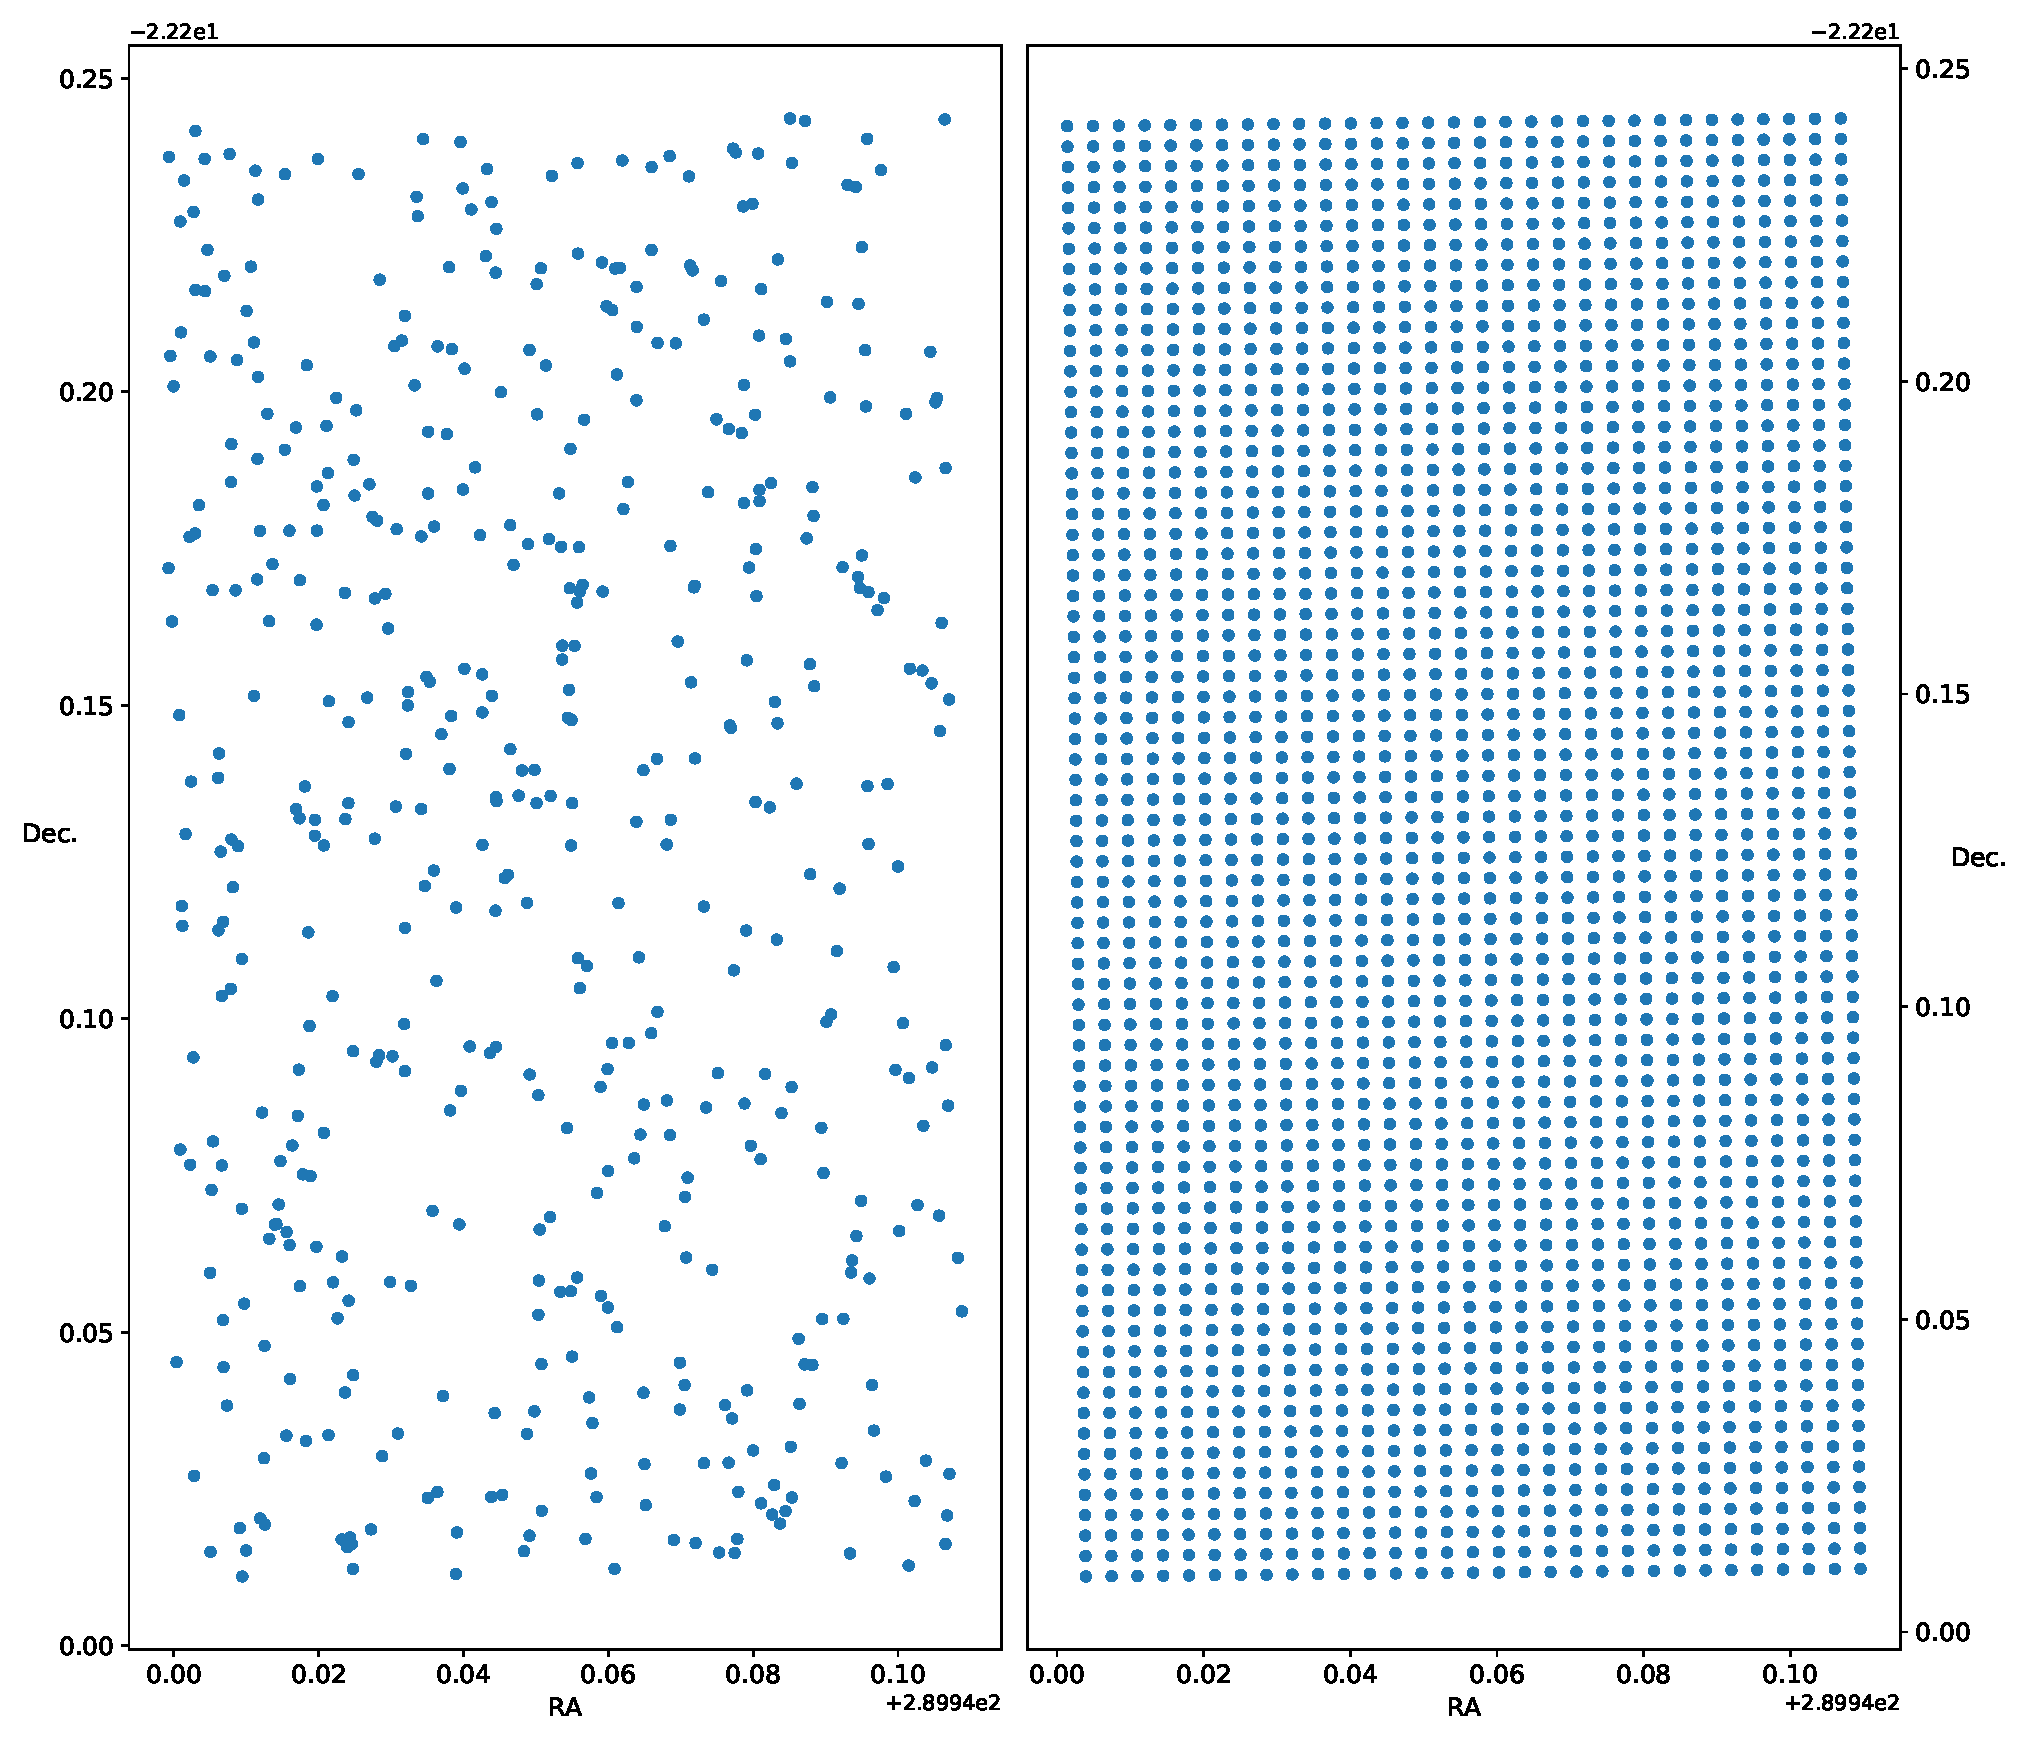
\includegraphics[width=\textwidth,keepaspectratio]{Figures/grid.pdf}
    \caption{This figure shows sky coordinates of centres where images are cut into 64$\times$64 pixel sub-images.
    The left plot has 500 randomized cutting positions and the positions were different for each FITS file pair, and the right plot has evenly spaced cutting positions with 63 pixel gaps.
    The left one is to have a randomized training/validation set with a less volume, and the right one is to retrieve the most planted and non-planted TNOs by searching the whole area.}
    \label{fig:grid}
\end{figure}

To generate the sub-images, the pixel coordinate on the first image pair is converted to sky coordinates and the second sub-image is centred at that sky-location, ensuring the two sub-images are of the same location on the sky.
For example, if the first element of time pairs was (2, 33), we then generated 500 pairs of sub-images from the 2nd and 33rd FITS files (which are separated by about 2 hours) with the centres of the sub-images taken from the randomized grid list locations in the 2nd image and the same centres of the sub-images in the 33rd image. The randomized centres changed for each time pair.

Each data set presented here is labelled by the number of the CCD from which it has been drawn.  For example, the sub-images made from the 20th CCD are labelled ``C20 images.'' 
A global training set was constructed by the concatenation of the C05, C10, and C20 data sets (combined data from multiple CCDs).  
This global data set provides artificial TNOs that had been made with a broader range of PSF models. 
Providing a number of different PSF shapes to guard against the model being trained to recognized the shape/structure of the artificial sources rather than the motion of the sources.
The combined data sets ``C051020'' was used as the main data set for training and testing the performance of our model.

We also created sub-samples for each CCD group of images based on selecting for training only those images that contained a TNO brighter than some limiting magnitude or images that did not contain a TNO.
For example, the data set labeled ``C20M23'' contains only those 64$\times$64 sub-images that contain a TNO brighter than the 23th magnitude as well as an equal number of sub-image pairs that do not contain a TNO.

For the implementation section, sub-images from the whole grid were used. 
In the Figure \ref{fig:grid}, the sampling difference between the training sets and testing sets are shown. 
Unlike the randomized sub-image centre positions on the left plot, the gaps between centre positions are constantly 63 pixels and the sub-images cover the whole CCD plane. 
The step between sub-images was set at 1 pixel smaller than the 64$\times$64 pixel sub-image to avoid an edge problem, which is a problem of having a moving object right at the edge of a sub-image.  This full data set is used to evaluate the detection efficiency of our algorithm.


\begin{deluxetable}{l|cccc}
  \caption{Examples of CFHT Megacam datasets names used in this research}
  \label{tab:Datasets}
\tablehead{
 \colhead{} & \colhead{5th CCD} & \colhead{10th CCD} & \colhead{20th CCD}& \colhead{5th+10th+20th}
 }
\startdata
    23th Magnitude & C05M23 & C10M23  & C20M23 & C051020M23\\ 
    25th Magnitude & C05M25 & C10M25 & C20M25 & C051020M25\\  
    27th Magnitude & C05M27 & C10M27 & C20M27 & C051020M27\\
\enddata
\end{deluxetable}

In summary, for training sets, we used FITS files from three CCDs (The 5, 10, and 20th CCD) to generate two-channel sub-images at randomized positions on the image.
The sub-image sets from the nth CCD was named as ``CnM27'', and its sub-samples containing only bright ones are named as ``CnM23'' or ``CnM25'', while the 23, 25, and 27 means the maximum magnitude of planted objects in the sub-image sets.
A data set made from concatenating C05, C10, and C20 were made as well and was named as ``C051020.''
Table~\ref{tab:Datasets} provides the names of data sets, and Figure~\ref{fig:magexamples} shows the examples of sub-images containing TNOs with magnitudes between 22 and 27.
%Furthermore, all training data sets were balanced to have same number of negatives and positives and thus the model does not go on a easy path, which is predicting everything negative or positive.

Testing requires presenting to the model data that has not been used for training and validation. Our testing data set consists of sub-images from all other CCDs not used in the training/validation process. 

\begin{figure}[ht]
    \centering
    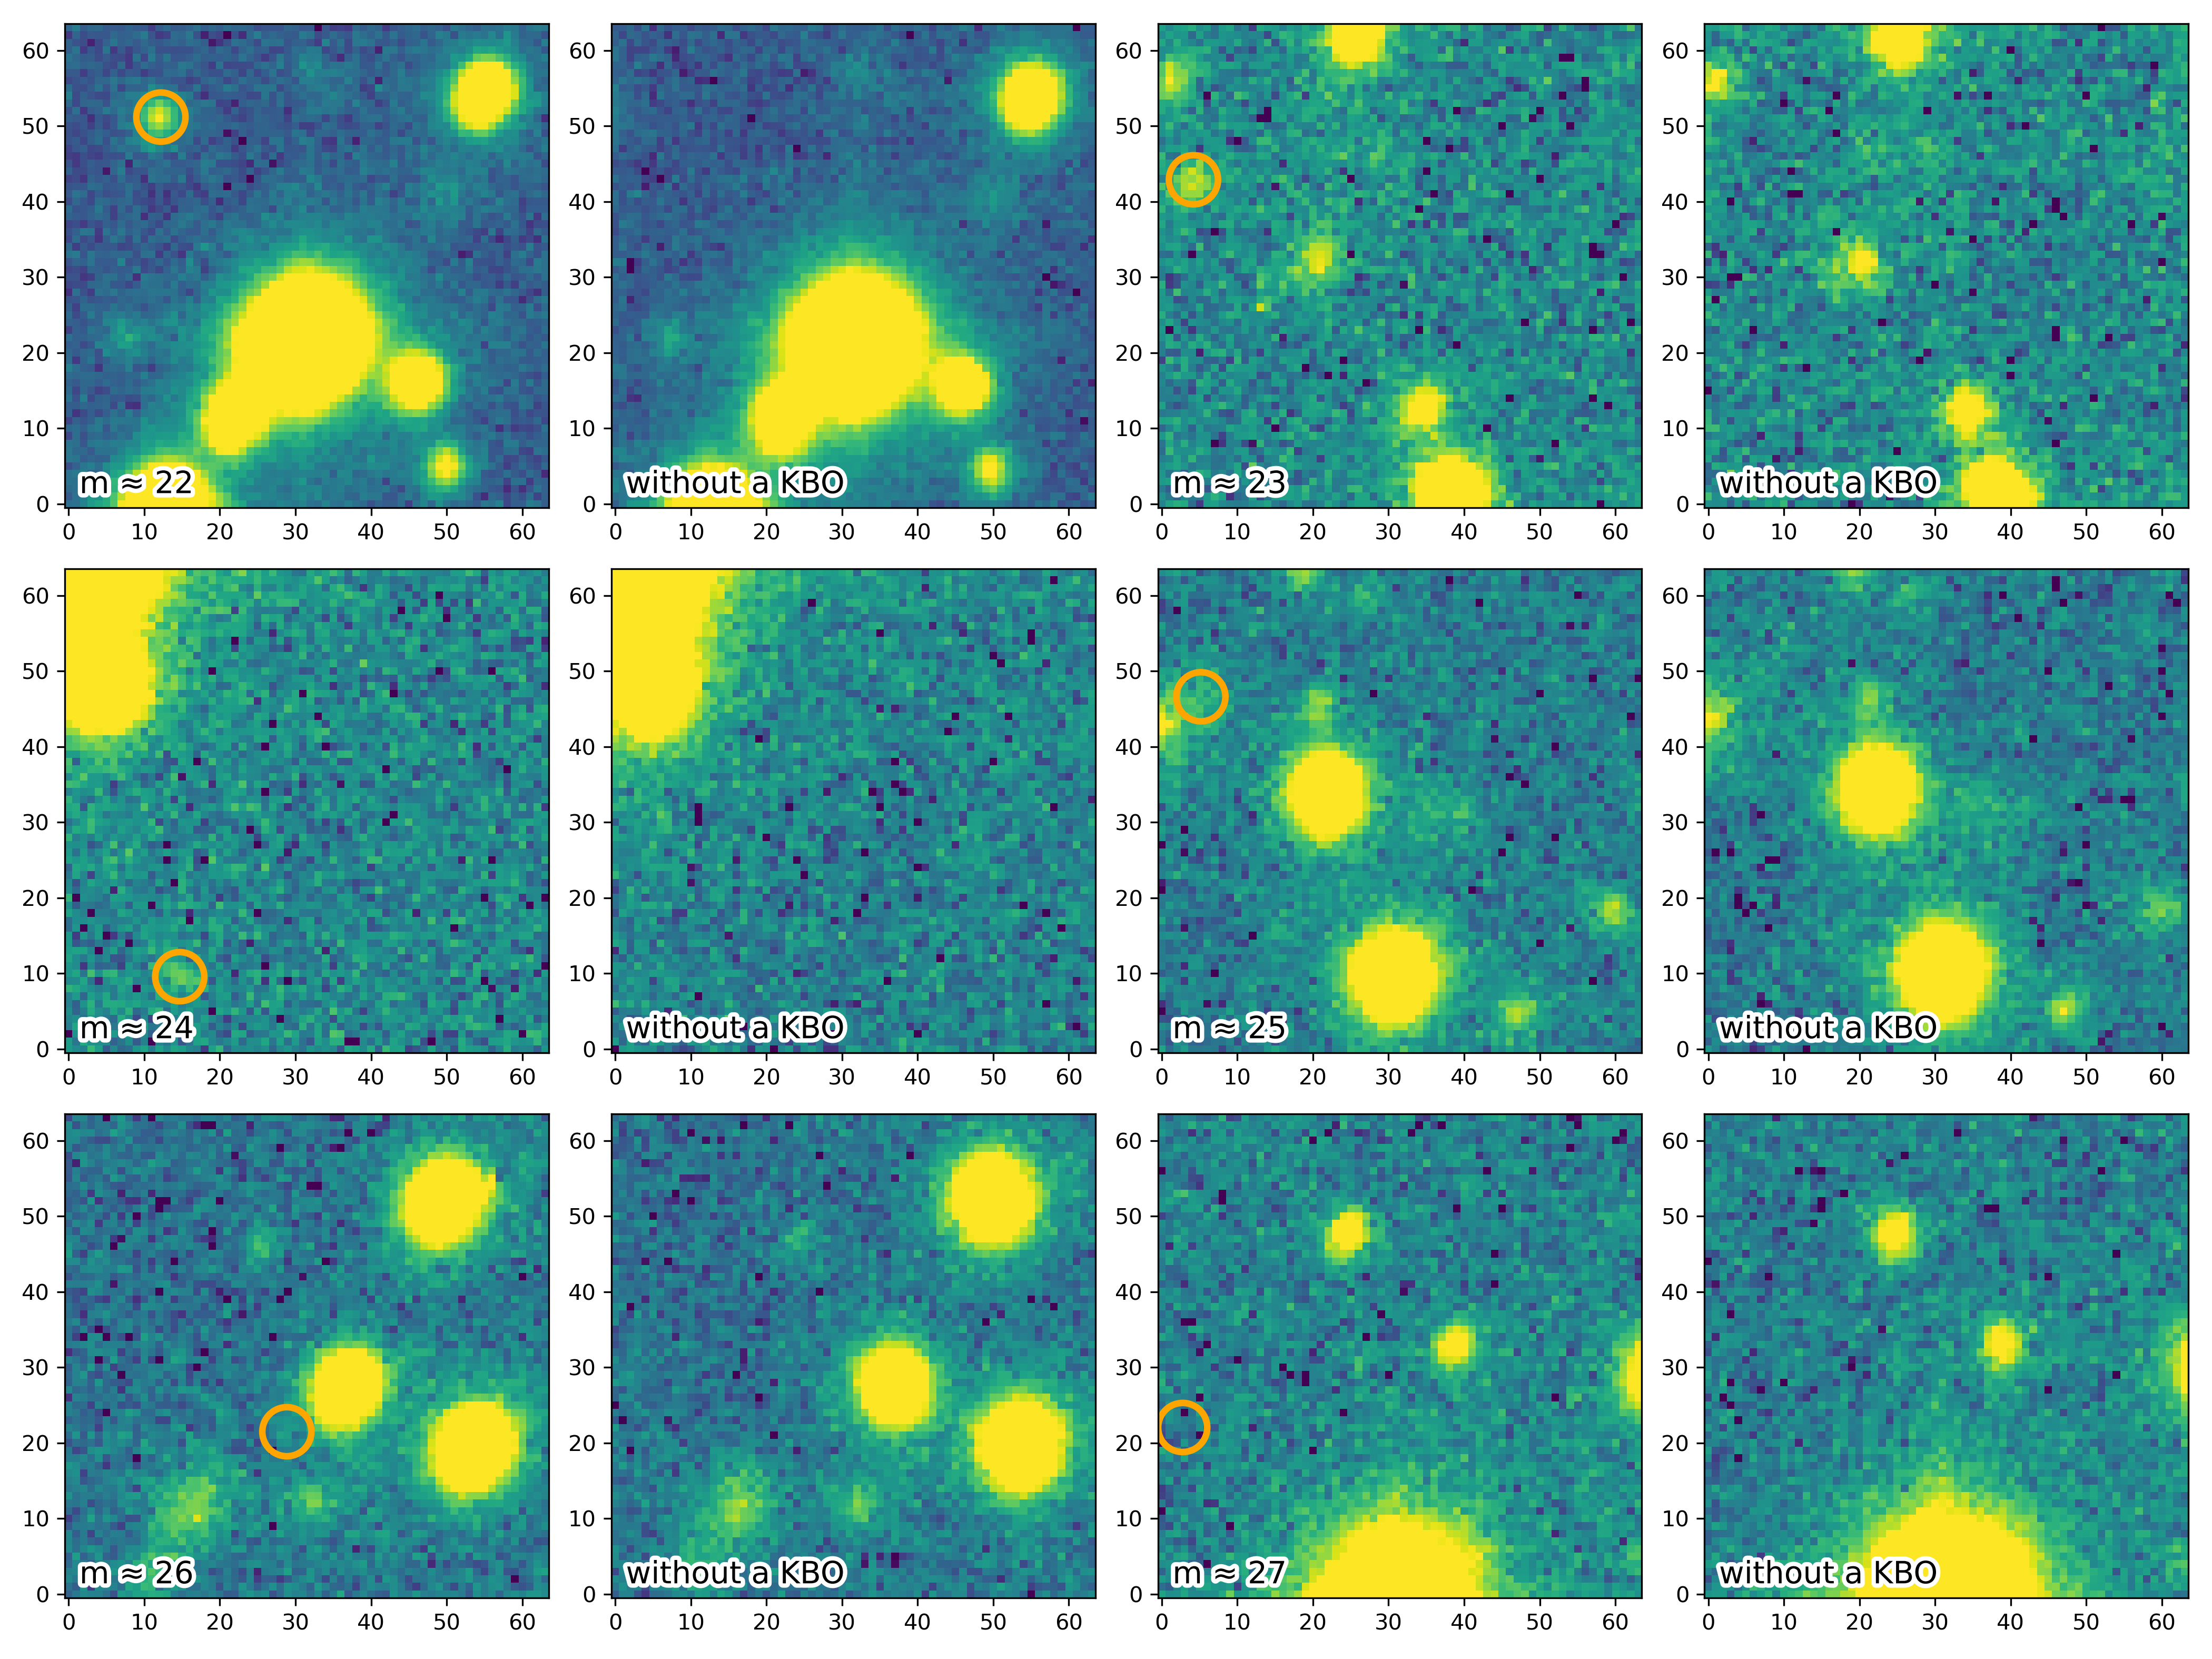
\includegraphics[width=\textwidth,keepaspectratio]{Figures/mag_examples.png}
    \caption{This figures shows 6 pairs of sub-images.
    Examples of sub-images used as our inputs. 
    The orange circle markers the location of the synthetic TNOs.
    From the left upper pair to the lower right pair, 6 pairs of positive-negative sub-images are shown.
    For the magnitude 22, 23 and 24 cases one can see the bright source in the positive sub-image that is absent in the negative sub-image taken from a different epoch.
    The magnitude 25, 26 and 27 sources are progressively more difficult to distinguish. 
    The artificial sources range from magnitude 22 to 27.}
    \label{fig:magexamples}
\end{figure}{}

\subsection{Labels}
\label{subsect:labeling}
Supervised learning requires labels attached to input data. 
The input data consists of the sub-images described in section \ref{subsect:subsets}, and the label for each sub-image indicates the presence of an artificial TNO in that sub-image.  
Sub-images containing an artificial TNO were labeled ``1'' while sub-images that do not have a TNO were labeled ``0.'' 
The labelling for classification was binary.
For example, the first two images on the upper left of the Fig \ref{fig:magexamples} are from the same sky coordinates.
The left image has a TNO of m$\approx$22, and the right image does not have a TNO. 
Therefore the pair of images would have (1, 0) as the label of classification.

In addition to a classification model, we trained regression models to determine the location and magnitude of the TNO to be used after the classification step.
To achieve this, each sub-image had labels holding the position and brightness of the TNO in the image.
This augmented information was not used by the classification model and is only made available to train a regression model which provides the position of the TNO within images classified as containing an object.
Since images were 64$\times$64 pixel size, those images were were labelled with x and y positions values between 0 and 64 and with apparent magnitude values between 22 and 27.
As a result, each sub-image on the first channel and the second channel was labeled with (p1, p2) for the existence of a TNO, and (x1, y1, x2, y2) for x and y coordinates of the TNO, and (m) for the magnitude of the TNO.

\section{Model Selection}
\label{sect: Model Selection}
The performance of predicting existence of a moving source in sub-images varies by the architecture and according to the training and validation set used.
Here we present a summary of results from our exploration of various combinations of models, training and validation sets.
 
\subsection{Architecture comparison}
\label{subsect:Architecture comparison}
Our initial examination looked at that the overall performance of our set of machine learning models.
%For this section we examine the performance of the model when trained and tested against various data sets previously created in the section \ref{subsect:subsets}.
To measure performance we need to determine the rate at which the model detects moving sources in our data.  
We intentionally added moving source that are well below the single exposure detection threshold as we wish to explore if our detection process can reach deeper into the data than more traditional approaches.
If we used source that are well bellow the detection threshold in measuring the performance of the model, however, we are not providing a realistic evaluation of the accuracy of our models.
The data sets for performance comparison only included sources brighter the r$<$25 magnitude (which is approximately the single-image detection threshold of our data set).  
Our performance testing is used to select, from those networks tested, the neural network that is most effective for our particular image classification and position determination problem.

\subsubsection{Classification} 
\label{subsubsect: Classification}

We present the performance and characteristics of the networks we tested in terms of: number of parameters; recall; precision; F1 score; number of true positives (TP); number of false positives (FP); number of false negatives (FN); and number of true negatives (TN), see in Table~\ref{tab:Classifier Comparison}.
All Metrics shown on the table were metrics when the classification threshold was set to be 0.5 (p values from the classification model must be larger than 0.5 to classify the images into positives).
Among these metrics, the recall indicates how well the models retrieve (detected) the artificial sources in the data set, recall is the primary metric of interest for our detection system.
Precision indicates how well the models exclude false positives out of all positively classified cases.
The precision is slightly less important than the recall because the false positives can be filtered using postprecessing and visual inspection at later stages of this method (section \ref{sect: Implementation}).
However, the precision is still an  important metric because a low precision rate would create a high visual inspection burden. 
Those two metrics introduced above can be expressed as the harmonic mean, the F1 score,
Which can be used as a single number to express both recall and precision metrics. The metrics are defined as:\\
\begin{equation}
    \label{eq:rpf}
    recall = \frac{TP}{TP+FN},\:\:precision=\frac{TP}{TP+FP},\:\textrm{and}\:\:F1 = \frac{2}{\frac{1}{recall}+\frac{1}{precision}}.
\end{equation}

\begin{deluxetable}{l|r|rrr|rrrr}
 \label{tab:Classifier Comparison}
  \caption{Classification performance of tested networks, based on the C051020M25 validation set.
  ``Param.'' is the number of parameters in each model, and other metrics are explained in section \ref{subsubsect: Classification}. Larger is better for recall, precision, and F1.}
\tablehead{
 \colhead{Architecture} & \colhead{Param.} & \colhead{Recall} & \colhead{Precision}& \colhead{F1} & \colhead{TP} & \colhead{FP} & \colhead{FN} & \colhead{TN}
 }
\startdata
    FCNN & 2.2M & 0.00 & 0.00 & 0.00 & 0 & 0 & 120045 & 119955\\
%    AlexNet-like & 2.8M & 0.787 & 0.879 & 0.830 & 94414 & 12986 & 25631 & 106969\\ 
    AlexNet-like & 2.8M & 0.79 & 0.88 & 0.83 & 94414 & 12986 & 25631 & 106969\\ 
%    VGG-like & 0.86M & 0.824 & 0.901 & 0.861 &98915&10824&21130&109131\\  
    VGG-like & 0.86M & 0.82 & 0.90 & 0.86 &98915&10824&21130&109131\\  
%    ResNet50 & 23M & 0.934 & 0.932 & 0.933  &112156&8166&7929&111749\\
    ResNet50 & 23M & 0.93 & 0.93 & 0.93  &112156&8166&7929&111749\\
%    ResNet50V2 & 24M & 0.900 & 0.957 & 0.928 &108105&4877&11980&115038\\
    ResNet50V2 & 24M & 0.90 & 0.96 & 0.93 &108105&4877&11980&115038\\
%    MobileNet & 3.2M & 0.913 & 0.917 & 0.915 &109631&9978&10454&109937\\
    MobileNet & 3.2M & 0.91 & 0.92 & 0.92 &109631&9978&10454&109937\\
%    MobileNetV2 & 2.3M & 0.914 &  0.885 & 0.900 &  109708 & 14212 & 10335 & 105745\\
    MobileNetV2 & 2.3M & 0.91 &  0.89 & 0.90 &  109708 & 14212 & 10335 & 105745\\
\enddata
\end{deluxetable}

% Timestamp: 2022-09-10

There was a strong variation in the performance of the different models.
FCNN failed to perform the image recognition task by classifying all image pairs to negatives.
The CNN architectures are made for 2D image recognition tasks and even a simple architecture such as AlexNet and VGG could be trained on our data set and classify the data set with recalls of approximately 80\%.

After we checked the capability of CNN-based networks on our data set, we proceeded with more complicated networks.
The ResNet50 and MobileNet architectures were our choices, and they were automatically modified for our input shape.
They showed better performance than AlexNet and a VGG with recalls of higher than 90\%.
ResNet50V2 and MobileNetV2 showed similar performance to ResNet50 and MobileNet. 
ResNet, MobileNet and their V2 networks provided us good enough performance to achieve our goals.

The recall and precision values reported in Table~\ref{tab:Classifier Comparison} are computed for a classification threshold of p$>$0.5. 
% The threshold means the reference point at which it is classified. 
% In this study, the threshold is the reference point for determining the presence or absence of TNO.
Recall and precision values are traded-off against the likelihood value used for classification. 
For example, if we set a higher threshold, the precision would go up, but the recall would go down. 
The threshold can be adjusted to achieve the highest model utility for the experimental setting. 
In other words, if TNOs detection per image is not critical but false positives are problematic we might set a higher threshold and regard precision to be more important than recall. 
If however we need to maximize detection even at the expense of a higher visual inspection burden, we can set a lower threshold and regard recall to be more important than precision. 
The impact on the overall detection efficiency caused by adjusting the threshold is illustrated in Figure~\ref{fig:completeness single}.

\begin{deluxetable}{l|r|rrrrrr}
  \caption{Regression performance on C051020M25 validation set. `Pos.' and `mag` columns refer to positional and magnitude uncertainties.  `MAE': Mean Absolute Error. `RMSE': Root Mean Square Error. Lower values indicate better performance.}
  \label{tab:Regressor Comparison}
  \tablehead{\colhead{Architecture} & \colhead{Param.} & \colhead{Pos. MAE} & \colhead{Pos. RMSE} & \colhead{Mag. MAE} & \colhead{Mag. RMSE}}
  \startdata
    FCNN &4.3M&10.5&16.0&1.8&3.0\\
    AlexNet-like &4.0M&1.6&5.3&0.2&0.3\\ 
    VGG-like &1.4M&5.8&6.9&0.2&0.3\\  
    ResNet50 & 24M&0.8&3.7&0.1&0.2\\  
    ResNet50V2 & 24M&0.8&3.9&0.1&0.2 \\  
    MobileNet &3.2M&0.91&3.8&0.1&0.2\\
    MobileNetV2 &2.3M&3.2&7.1&0.3&0.5\\
  \enddata
\end{deluxetable}

\subsubsection{Regression} \label{subsubsect:FixedDataRgs}

The performance of predicting positions of TNOs also varied by architecture.
The performance and characteristics of the regressor in terms of the number of parameters, the mean absolute error (MAE), the root mean square error (RMSE) of source positions and brightness are given in Table~\ref{tab:Regressor Comparison}.
The FCNN guessed the location of the TNO almost randomly, but VGG showed an improvement in all metrics especially on magnitude prediction, and AlexNet could predict the positions far better than we expected.
With this promising performance of CNN-based networks, we proceeded to explore ResNet and MobileNet.
ResNet50, ResNet50V2, and MobileNet predicted coordinates with an MAE less than one pixel and were found to be the best regressor architectures among those tested.
Interestingly, MobileNetV2 was worse at position prediction than MobileNet.

Out of architectures we have tested, we have chosen the MobileNet to be our architecture. 
MobileNet exhibits sufficiently high recall and precision when was used as a classifier, and low MAE and RMSE when used for regression. 
ResNet50 showed slightly better performance, but the difference was minimal but ResNet50 has 10 times the number of parameters and is more susceptible to over-fitting.
Additionally, MobileNet is highly efficient due to the smaller number of parameters.
Computational cost of predicting with MobileNet is relatively cheap compared to ResNet \citep{2020arXiv201108367S}.
Any number of advanced CNN-based networks could be suitable to our problem and continuing to explore these various architectures may reveal even better performance, but for our purposes the MobileNet network provides a good balance between performance and complexity.
For the remainder of this manuscript we adopted MobileNet. 

 \subsection{Training Data}
 \label{subsect:FixedArch}
 
After selecting a model we examined the nature of the training data and how the training data influences the model performance.

\setlength{\tabcolsep}{3pt}
\begin{deluxetable}{c|cc|cc|cc|cc|cc|cc}
  \label{tab:Single Chip}
  \caption{Classification performance on validation sets (same chip) and test sets (different chips) at p threshold=0.5.
  The table displays the performance of the models trained on an M25 data set.
  The models were validated/tested on a balanced M23 data set, which is a subset of the M25 validation/test sets, for a better presentation of their effectiveness on brighter objects.}
  \tablehead{\multicolumn{1}{c|}{Model} & \multicolumn{2}{c|}{Validation} & \multicolumn{2}{c}{Test 1 (C08)}& \multicolumn{2}{c}{Test 2 (C13)}& \multicolumn{2}{c}{Test 3 (C21)}& \multicolumn{2}{c}{Test 4 (C34)}& \multicolumn{2}{c}{Test avg.}\\
   & Recall & Prec. & Recall & Prec. & Recall & Prec. & Recall & Prec. & Recall & Prec.& Recall & Prec.}
   \startdata
%    C05&0.958&0.903&0.910&0.841 &0.899&0.880 &0.663&0.681 &0.660&0.657&0.783&0.765\\
%    C10&0.911& 0.902&0.904&0.820 &0.920&0.875 &0.725&0.681 &0.706&0.663&0.814&0.760\\
%    C20&0.903& 0.901&0.624&0.681 &0.630&0.652 &0.927&0.884 &0.894&0.871&0.769&0.772\\
    C05&0.96&0.90&0.91&0.84 &0.90&0.88 &0.66&0.68 &0.66&0.66&0.78&0.77\\
    C10&0.91& 0.90&0.90&0.82 &0.92&0.88 &0.72&0.68 &0.71&0.66&0.81&0.76\\
    C20&0.90& 0.90&0.62&0.68 &0.63&0.65 &0.93&0.89 &0.89&0.87&0.77&0.77
  \enddata
\end{deluxetable}

\subsubsection{Single CCD}\label{subsubsect:SingleCCDandMultipleCCDs}

First, we train and validate on a data set from a single CCD. For example, a training set based on 80\% of the entire C05M25 set and validation set based on 20\% of the C05M23 set.
By validating on the brightest data set we are exploring the networks ability to detect the moving source when sufficient signal is present in the data. 
Likewise, C10 and C20 models were also trained and validated. 
The ``validation'' column of Table \ref{tab:Single Chip} shows performance of each model on its validation set. 
The validation performance is fairly high for all sets.

However, when these models were tested on data sets from other chips, the classifiers were significantly less effective. 
For instance, the C05 model was effective to classify the C08 data set and C13 data set, but it was not effective for C21 data set and C34 data set. 
The network appears to be training on to characteristics specific to a particular CCD (perhaps the structure of the PSF).  
To improve the model performance requires an expanded training set.

\begin{deluxetable}{c|cc|cc|cc|cc|cc|cc}
\label{tab:Multiple Chips}
  \caption{Classification performance of the combined data set models on validation sets (same chip) and test sets (different chips) at p threshold=0.5.
  The table displays the performance of the models trained on an M25 data set when validated/tested on a balanced M23 data set.
  The suffixes ``R'' and ``M'' after the model names denote ResNet and MobileNet.}
  \tablehead{Model &  \multicolumn{2}{c|}{Validation} & \multicolumn{2}{c}{Test 1 (C08)}& \multicolumn{2}{c}{Test 2 (C13)}& \multicolumn{2}{c}{Test 3 (C21)}& \multicolumn{2}{c}{Test 4 (C34)}& \multicolumn{2}{c}{Test avg.}  \\
 & Recall & Prec. & Recall & Prec. & Recall & Prec. & Recall & Prec. & Recall & Prec.& Recall & Prec.}
 \startdata
%     C051020R & 0.976 & 0.938 & 0.906 & 0.888 & 0.920 & 0.922 & 0.931 & 0.899 & 0.894 & 0.879 & \textbf{0.913} & \textbf{0.897}\\
%    C051020M & 0.964 & 0.941 & 0.903 & 0.897 & 0.915 & 0.912 & 0.934 & 0.894 & 0.894 & 0.882 & \textbf{0.912} & \textbf{0.896}\\
    C051020R & 0.98 & 0.94 & 0.91 & 0.89 & 0.92 & 0.92 & 0.93 & 0.90 & 0.89 & 0.88 & \textbf{0.91} & \textbf{0.90}\\
    C051020M & 0.96 & 0.94 & 0.90 & 0.90 & 0.92 & 0.91 & 0.93 & 0.89 & 0.89 & 0.88 & \textbf{0.91} & \textbf{0.90}
\enddata
\end{deluxetable}

\begin{deluxetable}{c|cc|cc|cc|cc|cc|cc}
  \caption{Regression performance of the combined data set model on the validation set (same CCDs) and test sets (different CCDs) at threshold = 0.5.
  The table displays the performance of the models trained on an M25 data set when validated/tested on a balanced M23 data set.
  The suffixes ``R'' and ``M'' after the model names denote ResNet and MobileNet.}
  \label{tab:Multiple Chips Regressor}
  \tablehead{Model &  \multicolumn{2}{c|}{Validation} & \multicolumn{2}{c}{Test 1 (C08)}& \multicolumn{2}{c}{Test 2 (C13)}& \multicolumn{2}{c}{Test 3 (C21)}& \multicolumn{2}{c}{Test 4 (C34)}& \multicolumn{2}{c}{Test avg.}\\  
 & pos. & mag. & pos. & mag. & pos. & mag. & pos. & mag. & pos. & mag. & pos. & mag.}
\startdata
%    C051020R & 0.408 & 0.0798 & 1.89 & 0.198 & 1.55 & 0.188 & 1.30 & 0.145 & 1.34 & 0.178 & \textbf{1.52} & \textbf{0.177}\\
%    C051020M & 0.500 & 0.103 & 1.88 & 0.208 & 1.56 & 0.208 & 1.34 & 0.178 & 1.87 & 0.209 & \textbf{1.66} & \textbf{0.201}\\
    C051020R & 0.41 & 0.08 & 1.9 & 0.2 & 1.6 & 0.2 & 1.3 & 0.1 & 1.3 & 0.2 & \textbf{1.5} & \textbf{0.18}\\
    C051020M & 0.5 & 0.1 & 1.9 & 0.2 & 1.6 & 0.2 & 1.3 & 0.2 & 1.9 & 0.2 & \textbf{1.7} & \textbf{0.2}
\enddata
\end{deluxetable}

\subsubsection{Multiple CCD}
\label{subsubsect:MultipleChips}

\begin{figure}[ht]
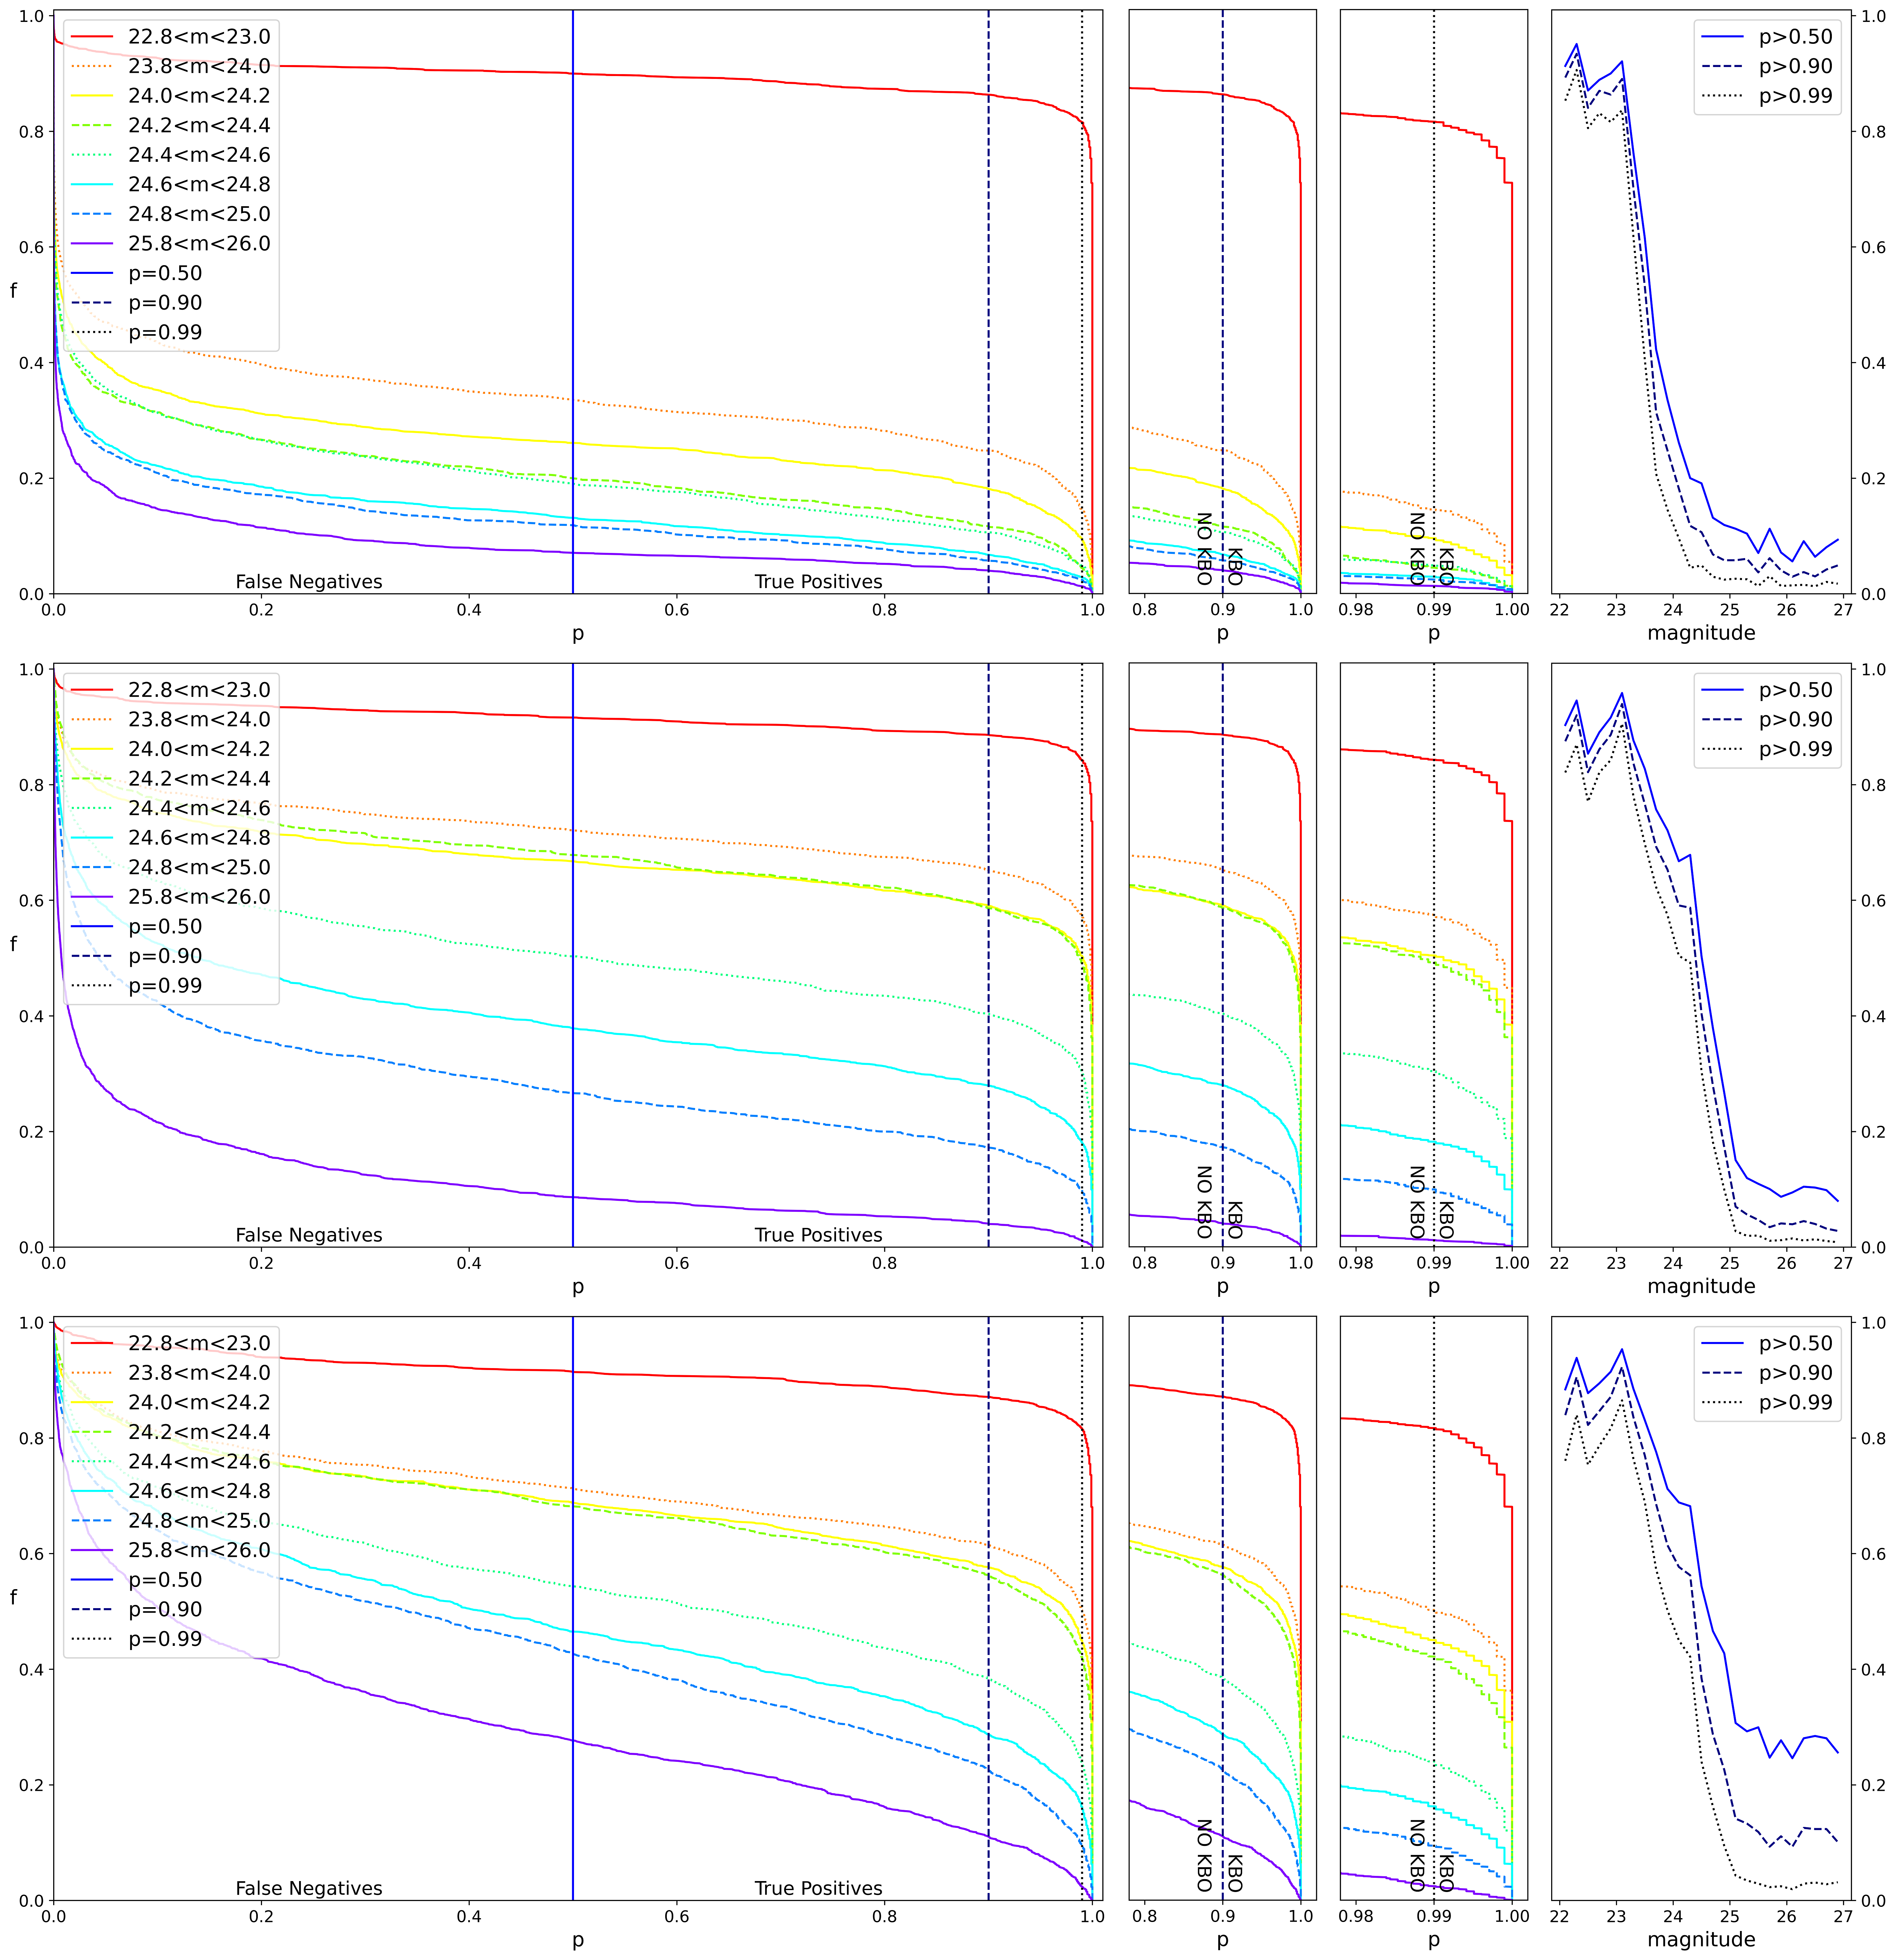
\includegraphics[width=\textwidth,keepaspectratio]{Figures/completeness_positives.png} \caption{Cumulative plots of detection efficiency of the MobileNet model trained using different input data sets.
Upper: Trained on data with sources brighter than m=23. centre: m=25. Lower: m=27.
On the left side of each panel, shows classification probability (p) versus fraction (f) of sources with a moving source correctly classified. 
The vertical blue/navy/black lines shows various thresholds that can be used to select images that may contain a moving source.
Thresholds of 0.5, 0.9, and 0.99 are shown.
The middle panels show the classification behavior near the 0.9 and 0.99 thresholds.
The panels in the right column show the fraction of sources correctly classified as a function of the brightness of the source, also know as the completeness curve. \label{fig:completeness single}} 
\end{figure}

\begin{figure}[ht]
    \centering
    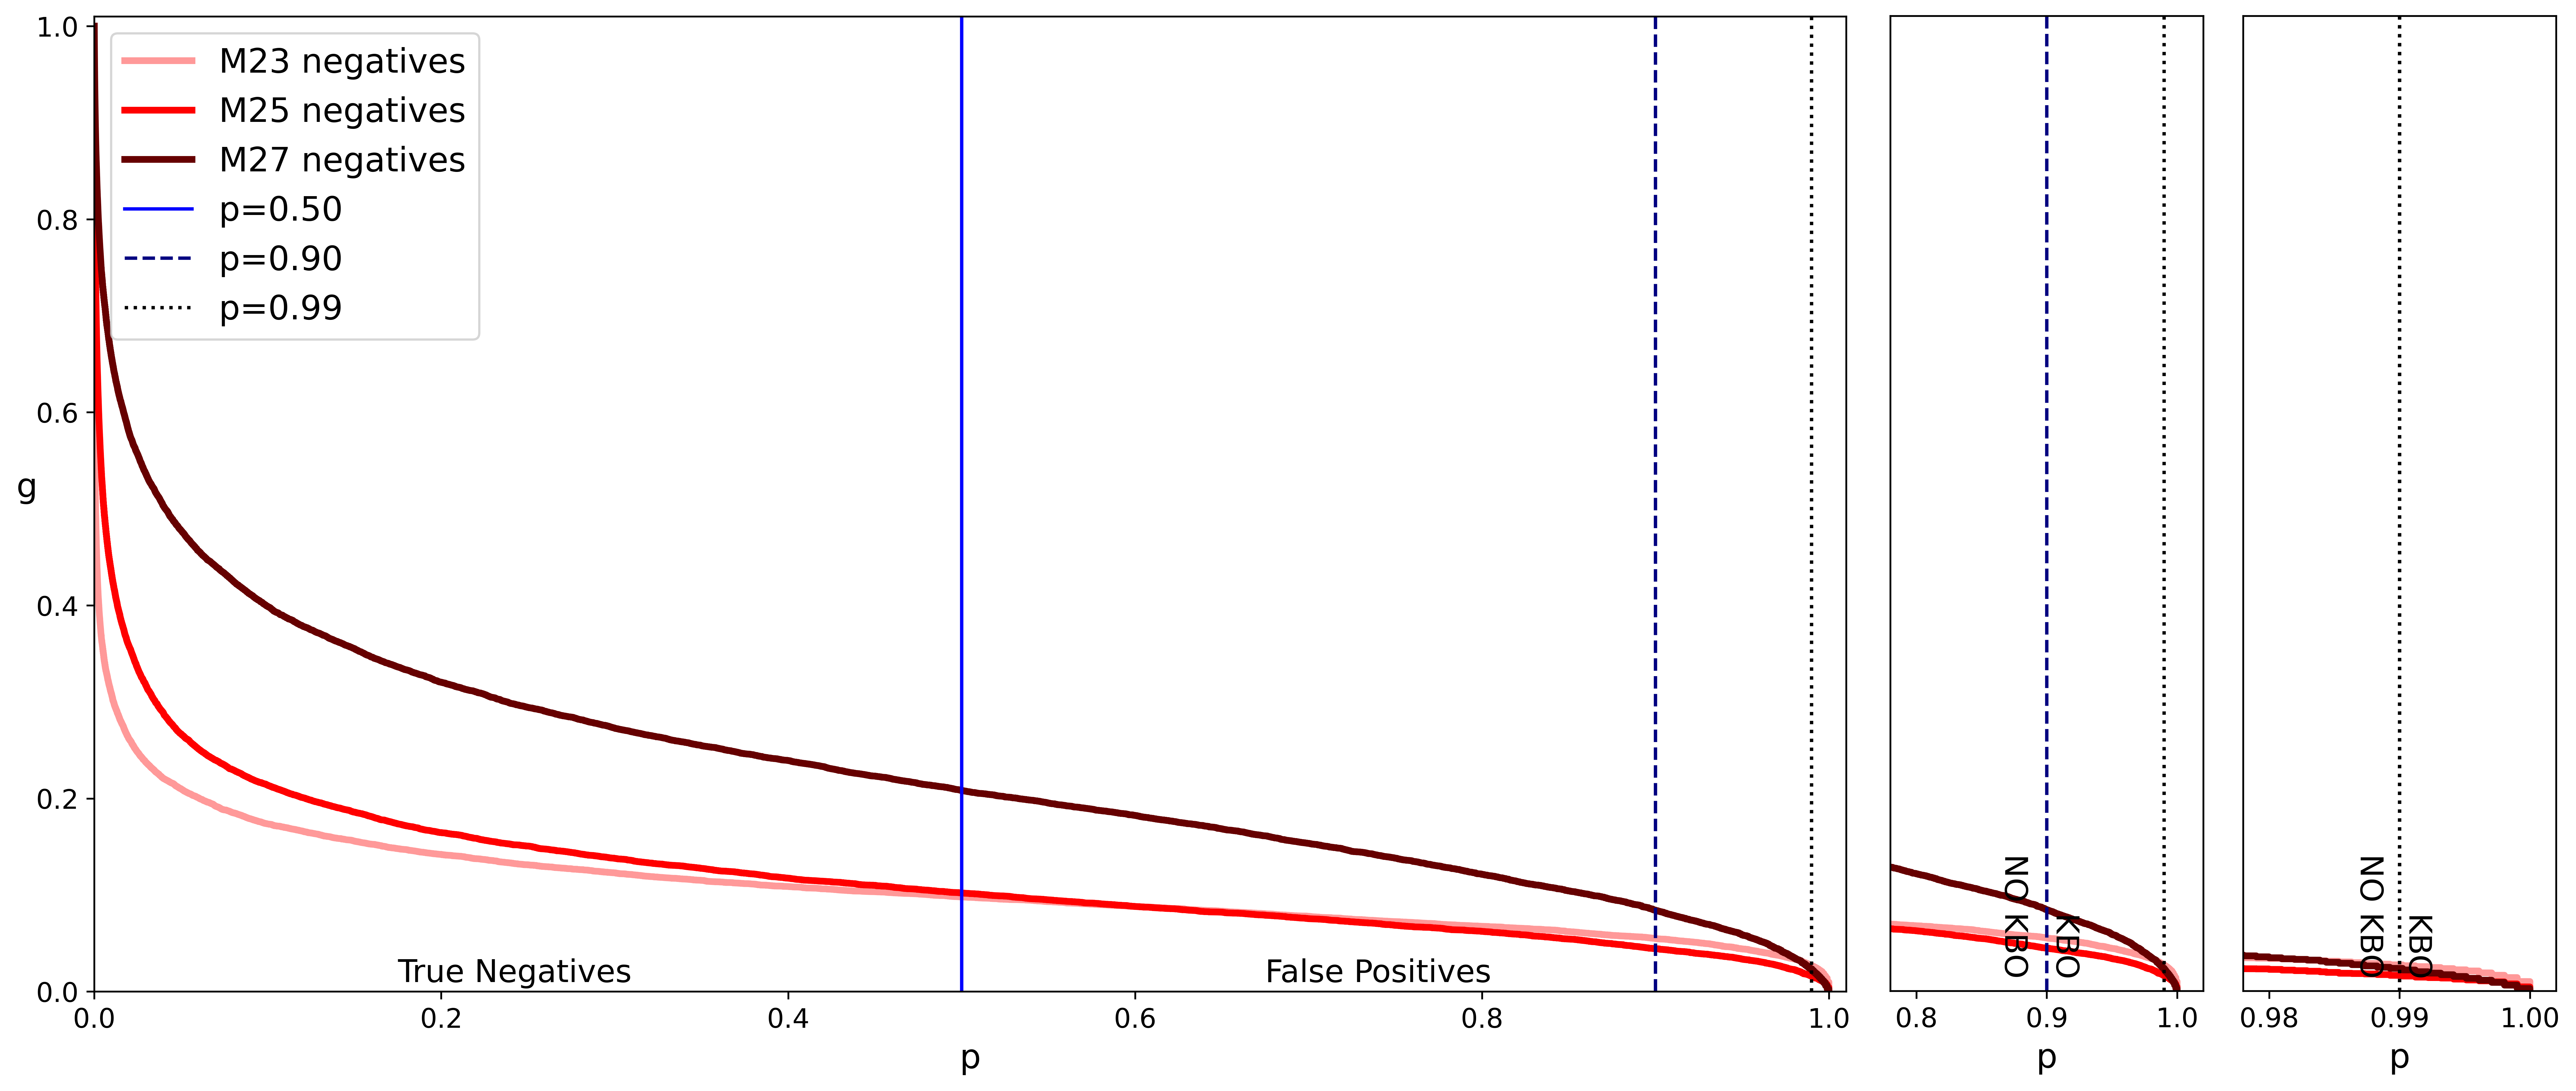
\includegraphics[width=\textwidth,keepaspectratio]{Figures/completeness_negatives.png}
    \caption{Cumulative plots of model probability (p) versus fraction of images classified as  containing a moving source (g).  
    All image pairs used for this plot are negatives, i.e. do not contain any artificial moving sources.
    Thus, g is the number of false positives compared to the total number of negative sub-images.
    There is very little difference between the M23 and M25 false-positive rates.
    The M27 model, however, returns false positives at double the rate of the M23/M25 models when p=0.5.}
    \label{fig:negatives}
\end{figure}
\setlength{\tabcolsep}{6pt}

\begin{figure}[ht]
    \centering
    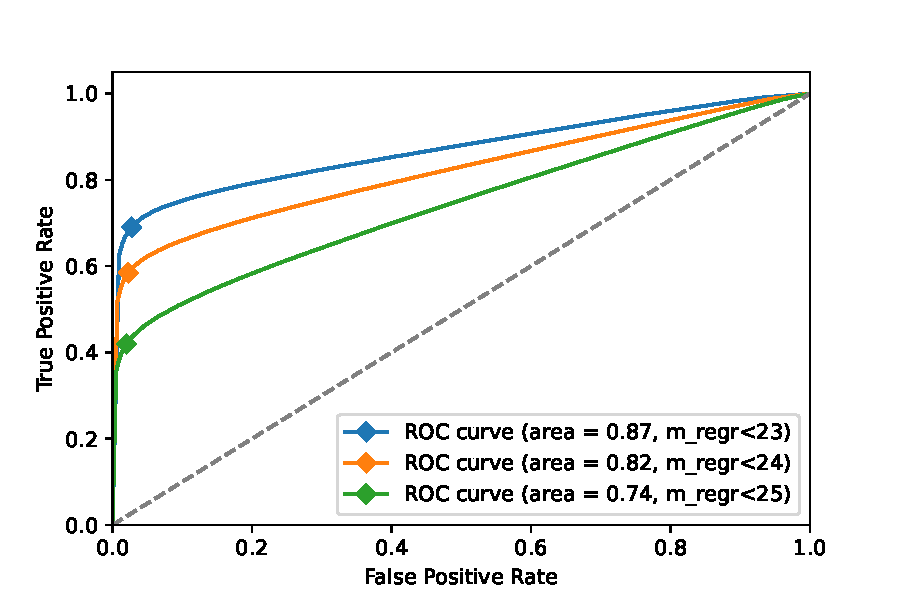
\includegraphics[width=0.6\textwidth,keepaspectratio]{Figures/ROC.pdf}
    \caption{ROC curves from testing the C051020M25 classifier on image pairs.
    The x-axis is the false positive rate that shows how frequent false alarms are compared to the total number of negatives (Less is better).
    The y-axis is the true positive rate that shows how many positives are correctly classified as positives compared to the total number of positives (More is better).
    These ROC curves show the general performance of the classifier when applied with various p thresholds.
    The more the curve is skewed to the left-upper area, the better the classifier performs.
    Area under curve (AUC) indicate the performance of the classification model (More is better).
    For example, if an ROC is the grey dashed line, it is random (AUC=0.5).
    The ROC curves have AUCs of 0.87, 0.82, and 0.74 depending on the maximum magnitude limits of 23, 24, and 25.
    The diamond markers show the points where when classification threshold p is at 0.99.
    }
    \label{fig:ROC}
\end{figure}

C051020, the combined data set described in section \ref{subsect:subsets}, provides a more diverse training set. 
The model trained on a single chip data set showed recall and precision mostly below 80\%. (see Table~\ref{tab:Single Chip})
When a MobileNet model was trained on C051020M25 data set, however, the test results on C08M23, C13M23, C21M23 and C34M23 data sets were evenly and sufficiently high at approximately 90\%.\footnote{There is no particular reason why the 5th, 10th, 20th CCD data sets are chosen for training, and the 8th, 13th, 21th, 34th CCD data set are chosen for testing, the choice of which CCDs to use for training and which to use for testing was made arbitrarily.} (see Table~\ref{tab:Multiple Chips})
Using the larger and more diverse training set appears to have removed our overfitting problem.
For the remainder of the manuscript we considered only the MobileNet model trained on the C051020 data set.

\subsubsection{Magnitude Limit on the Training Data}
\label{subsubsect: Magnitude Limit on the Training Data}
We have analyzed the M23, M25, M27 models to determine which magnitude limit on the training data gives the best result.
In the Figure \ref{fig:completeness single}, the completeness of each model trained on a combined test set C08132134 is shown.
M23 model was effective to classify a test set up to the 23th magnitude objects, and quickly became ineffective faint-ward of approximately 23.5: the model trained on bright sources could not predict the existence of a moving source significantly fainter than in the training set.
M25 model could classify images with objects brighter than the 23rd magnitude, similar to the M23 model.
But, the recall drops quickly fainter-ward of approximately 24.3 instead of approximately 23.5.
M27 model showed similar aspects to the M25 model.
Because the model was trained with a data set including up to the 27th magnitude objects, it could retrieve some of dim objects, but by using the M27 model to classify images, there was a problem that the fraction of false positives increases (see Figure~\ref{fig:negatives}).
The fraction of false positives compared to the total number of negative sub-images of the M27 Model, the fraction g on the Figure~\ref{fig:negatives}, was approximately 21\% when p=0.5, indicating a significant population of false positives would be included after the classification.
% We can use the p=0.99 to be our threshold to classify the positives and negatives, as Figure~\ref{fig:completeness single} shows that the classification behaviour of the M25 model at p=0.5, 0.9 and 0.99 are very similar.
Therefore, C051020M25 model can correctly classify images including faint sources as well as the M27 model but with fewer false positives than the M27 model.
The general performance of this model is shown with ROC curves on the figure \ref{fig:ROC}.
We concluded that the $\sim$24.5th magnitude is the limit we can successfully classify objects with this method, and we decided to use the C051020M25 MobileNet model going forward.

% Timestamp: 2022-09-15

\section{Implementation}
\label{sect: Implementation}
Given the trained and selected models, we now examine how these models can be used to discover SSOs.
The C051020M25 MobileNet classifier was our choice of classifier, and C051020M25 MobileNet regression model was our choice of predicting positions and magnitudes.
Requiring p$>$0.99 for our classification model correctly filters out $\sim$98\% of images without a moving source (see Figure~\ref{fig:negatives}.)
Even the 2\% leftover from the CNN classification, however, results in large number of false positives.
To further reduce the false positives, we investigated two kinds of postprocessing methods.

% \begin{figure}[ht]
% 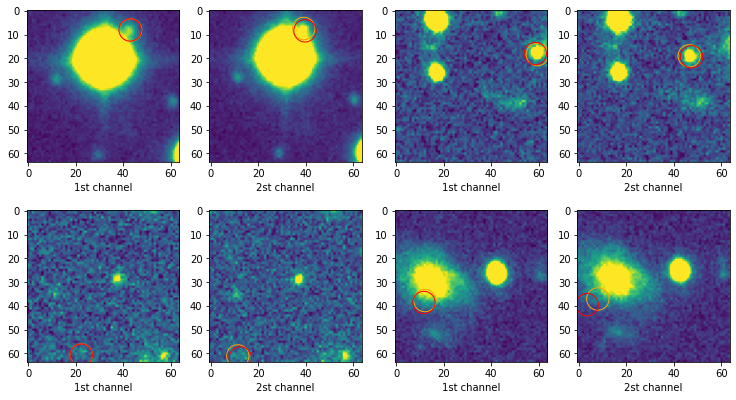
\includegraphics[width=\textwidth,keepaspectratio]{RegressionExamples.png}
% \caption{Examples of images with successfully classified image with measured positions.
% Orange circles are the real positions of TNOs, and the red circles are measured positions of TNOs.
% (Upper Left) A bright TNO (m $\approx$ 22) passing near a star.
% (Upper Right) A bright TNO (m $\approx$ 22) with a precise measurement.
% (Lower left) A dim TNO (m $\approx$ 25) with a successful detection.
% (Lower right) A dim TNO (m $\approx$ 25) with a wrong measurement of position.
% Even when the classification was made correctly, sometimes the measurement of positions could be wrong.
% \label{fig:Regression_examples}} 
% \end{figure}

\subsection{Approach 1: Linear Fitting Approach}
\label{Subsect: Linear Fitting Approach}
We first tried to use both classification model and regression model.
In this study, the classification model measures the likelihood that each image in a pair belongs to the ``has a TNO'' class.
The classification model provides likelihoods p1 and p2 between 0 and 1 and the user then selects at what level of likelihood an image is classified as containing a TNO. 
The choice of likelihood values is dependent on the goals and intentions of the specific project.
A project desiring to provide a very pure sample may require a threshold of p$>$0.99 while a project attempting to detect as many TNOs as possible might have a lower threshold value.
For example, if the threshold is 0.5, images with values above 0.5 will be classified as having a TNO but that may create a high false-positive rate. 
By adjusting the threshold like this, we decided how strictly we want to filter the proposed detection.
Classification models and regression models were trained on each data set and the models were stored separately.
After that, by adjusting the thresholds of the models, how performance metrics such as recall and precision change were identified and recorded.

Recall and precision can be used as criteria for classifier performance.
For example, if a classifier has a recall of 0.9 and a precision of 0.8, this means that the filtered data set will miss 10\% of the moving sources and 20\% of the predicted positives are actually negatives.

In reality, TNOs are scarce on the sky at the flux limits of this experiment (about 1 per CCD) and very few sub-images will have a real TNO. 
This results in the number of negatives classified as positive (false positives) being far greater than the number of true positives, unless the p threshold is very near to 1. 
This creates the problem that the number of false positives make TNO exploration practically impossible. 
From this sparseness of TNO, necessity of another postprocessing step emerged.

When the classification model declares (p$>$0.5) that a moving source is present in the sub-image we pass the two sub-images to the regression model which provides estimates of the (x1, y1, x2, y2) position of the moving source (see Table~\ref{tab:Regressor Comparison} for estimates of the precision of these estimates).
A distant solar system object, such as a TNO, will exhibit linearly sky motion over the short time period (a few hours) during which our data have been acquired. 
Multiple source detection within a small area of sky are likely to be of the same object and the rates of motion inferred by grouping these source measurements should be consistent with expectations for a solar system body. 
By requiring that each source measurement in a group is consistent with expected linear motion, and rejecting from the group those sources that are inconsistent with this behaviour, we are able to list the potential moving objects.

In detail, the linear motion of TNOs were detected in following steps.
First, for every single source in the data set, a list of sources that may be grouped as a single object, based on proximity on the sky, were built.
This results in the grouping a few dozens nearby sources measurements.
A maximum-likelihood based fit to linear motion, with iterative rejection of those sources that are more than 4-$\sigma$ from fit, was then performed.
Once an acceptable fit was determined, those source measurements that are within 0.5 arc-seconds of the linear model were accepted as belonging to the same candidate object (see Figure~\ref{fig:linking}).
Candidate objects with more than three source measurements (a triplet) and that exhibited rates of sky motion of between 0.5 and 15 arc-seconds per hour, reasonable rates for solar system bodies between 10~au and 300~au when observed at opposition, were then selected for visual inspection.

\begin{figure}[ht]
    \centering
    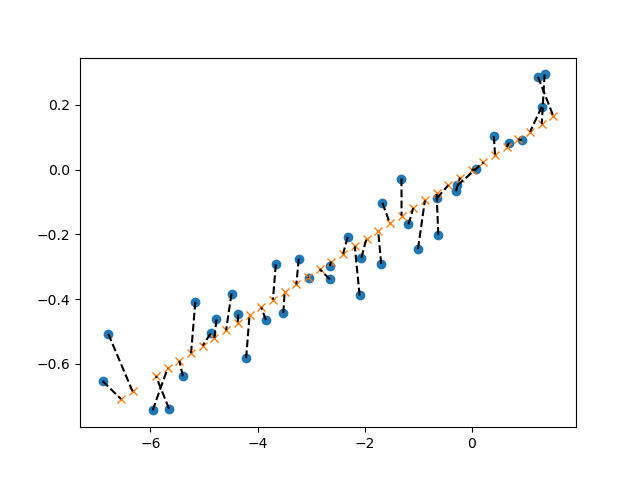
\includegraphics[width=0.6\textwidth,keepaspectratio]{Figures/diagnostic.png}
    \caption{Blue dots are regression-predicted positions of a group of sources that classification model gave p$>$0.5 probability of being a moving source. 
    Yellow crosses are the predicted locations a moving source would be at, in each exposure, based on a maximum likelihood-based linear fit to the regressor-based locations.
    The linear model provides an excellent match to this group of sources which are then declared as moving object candidates.
    }
    \label{fig:linking}
\end{figure}

% Hence, we can find only slow-moving objects such as TNOs, or find only fast-moving objects such as NEOs and asteroids, or find both of them.
% If the number of sources in the list was less than a certain number (in other words, if there are no nearby sources), the list of sources was excluded.
% Second, the moving rates toward the grouped nearby sources from the single source are calculated.
% If a moving rate is outside of a normal moving rate of TNO, or the predicted magnitude of nearby sources is far from the predicted magnitude of the single candidate source, the nearby sources is excluded from the list of sources.
% Again, if the number of sources is less than a certain number, the list itself is excluded.
% Third, with the candidate sources survived, fitting lines for predicted TNO positions and time of observation are modelled with following equations.
% Following is how we defined the model to find the best fitting starting position and time of the line, rate of motion and angle.

% \[ 
% RA_{model} = r_0 + rate \times (t - t_0) \times cos\:(angle)
% \]
% \[ 
% Dec_{model} = d_0 + rate \times (t - t_0) \times sin\:(angle)
% \]
% The log-likelihood function is defined as 
% \[
% ln\:L(\theta, r, d, t, \sigma_{RA}, \sigma_{Dec}) =
%     -\sum^{n}_{i=1}((RA_i - {RA_{model, i}})^2 /  {\sigma_{RA}}^2) -\sum^{n}_{i=1}((Dec_i - Dec_{model, i})^2 / {\sigma_{Dec}}^2) 
% \]
% where $\theta$, the values to be tuned, are $r_0$, $d_0$, $t_0$, rate, angle
% and $\sigma_{RA}$ = $\sigma_{Dec}$ = 0.1875 arcsec.

%We could fit the sources not only with their positions but also with their time of observation with this method.
%After this linear fitting, the nearby sources which are further than 0.5 arcsecond from the fitting line are excluded.
%Again, the list of sources with a number less than a certain number is excluded.

The linear fitting steps above filter out many of the false positives from section \ref{Subsect: Linear Fitting Approach} by only accepting sources that can be linearly connected into linked sources and with linear rates of motion that are consistent with expectation for solar system bodies.
We call the accepted linked sources a candidate ``track''. 
The maximum number of sources measurements in a single track is 44, as there were 44 images in our input time series.

% Because the position predicting is not perfect and does not always satisfy the proximity, magnitude, and rate of motion requirements, this process could not track all sources from a planted TNO.
% We could make the list of TNO candidates with this process, and the number of list of non-planted sources are left to the visual inspection.

%This tracking process is a Postprocessing process using the predictions from the regression model and at the same time it is a process to find the orbits of TNOs.
%We can have (RA, Dec) positions of candidate detections converted from (x1, y1) positions and also obtain orbital elements from tracklets.
% The rate and angle of the motion can provide rough estimates of the distance to the TNO and its angle of motion on the sky.
% Grouping the multiple measurements together that form a track we could proceed to determine Keplarian orbital elements that are consistent with the observed sky motion, Even in the optimal case, however, the orbital elements of TNOs determined from a 2 hour observed arc will be highly imprecise and we did not pursue the precise orbit on this analysis.

After this fitting process, there is still a possibility that non-SSO images are passed as a SSO candidate.
This occurs when there is a defect, such as saturation bleed, in the image and this defect moves slightly from exposure to exposure in a way that mimics an SSO.
Hence, a visual inspection is made for the final candidate selection.
The inspection consists of examining the scatter plot of the candidate track (For example, Figure~\ref{fig:linking}) and confirming or rejecting the existence of a moving object in the image in the associated sub-images.

% After the visual inspection, we realized that this approach gave us only half success because inspecting tracks did not result in a high number of visibly bright non-planted SSOs.
% After the brief inspection over tracks with n$\geq$9, we found two slow SSOs the rate of moving objects was 1-3 arcsecond/hour.
% Other than those two slow SSOs, tracks did not contain other visually bright real SSOs.
% This approach worked on planted slow-moving TNOs, but it did not yield the number of non-planted TNOs we expected from our data set.

After a brief visual inspection, we found that the MAE of the regression model result for faint objects ($m\geq23$) is too large to enable accurate linear fitting.
Moreover, while some TNOs were successfully detected, we could only find very few real SSOs or TNOs because of confusion caused by densely populated planted sources.
Therefore, we explored another way to exploit the CNNs.

\subsection{Approach 2: Scoring Approach}
\label{subsect: Scoring Approach}

This time, we attempted to use only the classification model.
The output of the classification model is (p1, p2).
For each series of sub-images at the same coordinates, we gave them a score by summing up p1 or p2.
For example, there are 44$\times$43 p's from measuring (1st=1st exposure, 2nd=2nd exposure), (1st, 3rd), (1st, 4th), ..., (2nd, 3rd), (2nd, 4th), ..., (43th, 44th) image pairs with the classification model at fixed coordinates (x1, y1).
We excluded p's less than 0.99, and hence most of false positives can be avoided.
Additionally, the value of p's were linearly mapped using the function: $\tilde{p} \coloneqq (x-0.99)\times100$. This function transformed the values from 0.99 to 0, from 0.991 to 0.1, from 0.992 to 0.2, ..., from 0.999 to 0.9, and from 1 to 1.
We sum the mapped $\tilde{p}$'s for each time-series sub-image sets.
This summed probability value, or a score, expresses a likelihood of having a moving source in the sub-image set.
In other words, the score is the likelihood to detect a moving source in the sub-images fixed at the same sky coordinate throughout the 44 images.
We ran this scoring on all sub-image sets, and excluded sets with a low score.

We also use the average of the original (unscaled) values of p for each exposure of a sub-image to filter the candidate list.
Each exposure sub-image is classified 43 separate times (once for each time that exposure appears in a sub-image pair).
The classification value, P, assigned to a given exposure sub-image is the average of the 43 classification values for that exposure sub-image.
For example, the sub-image for exposure i is paired with the 43 other exposure sub-images and presented to the CNN classifier.  
For each pair of sub-images, the classifier returns 2 values, one for each of the sub-images.  
We then take the value of P as the average of all values of p's that were returned for a given exposure (43 values). 
We observed that the P rarely goes above 0.85 if a moving object is not clearly present during visual inspection.
Therefore, we excluded sub-image series that do not have a P larger than 0.85.
After this step, only series that have a clear P spike remained.
In short, a time-series sub-image set should pass two conditions: $\sum^{all\:pairs}\Tilde{p}\geq$ 80 and $\exists P \in A : a \geq 0.85$ to be considered as a candidate.
This additional postprocessing step significantly decreased the number of false positives.

% And then, we can visually inspect image series with cumulative probabilities higher than a threshold.
% We confirmed this approach can find visibly bright non-planted SSOs far better than the previous linear fitting approach.

Candidates with more than a certain score were very likely to include a visible and obvious moving object.
Therefore, we might be able to claim that very highly scored sub-image series (For example, score$\geq$1000) include a SSO, without additional visual inspection.
Note that the maximum possible score was 44$\times$43=1892.
This automated feature can be very useful for a future survey as the detections of the survey can be reported rapidly.

Moreover, sub-image series with a high score (For example, 80$\leq$score$<$1000) can be further visually inspected to determine if they contain SSOs.
For the inspection, we made GIF animations with stretched and normalized pixel values and chose the time between each frame to be 125ms.
As an additional information to the image, the inspector was given the number of the current image frame (1 to 44) and the p average value attached to each sub-image series.
In this way, the inspector can estimate when the moving source appears during the inspection.
This additional information is quite helpful when the moving light source is faint.

% Timestamp: 2022-09-19

\section{Results and Discussion}
\label{sect: Results}

We present the results from two postprocessing approaches, show the peak detection efficacy, and finally show the real SSOs we found.

\begin{figure}
    \centering
    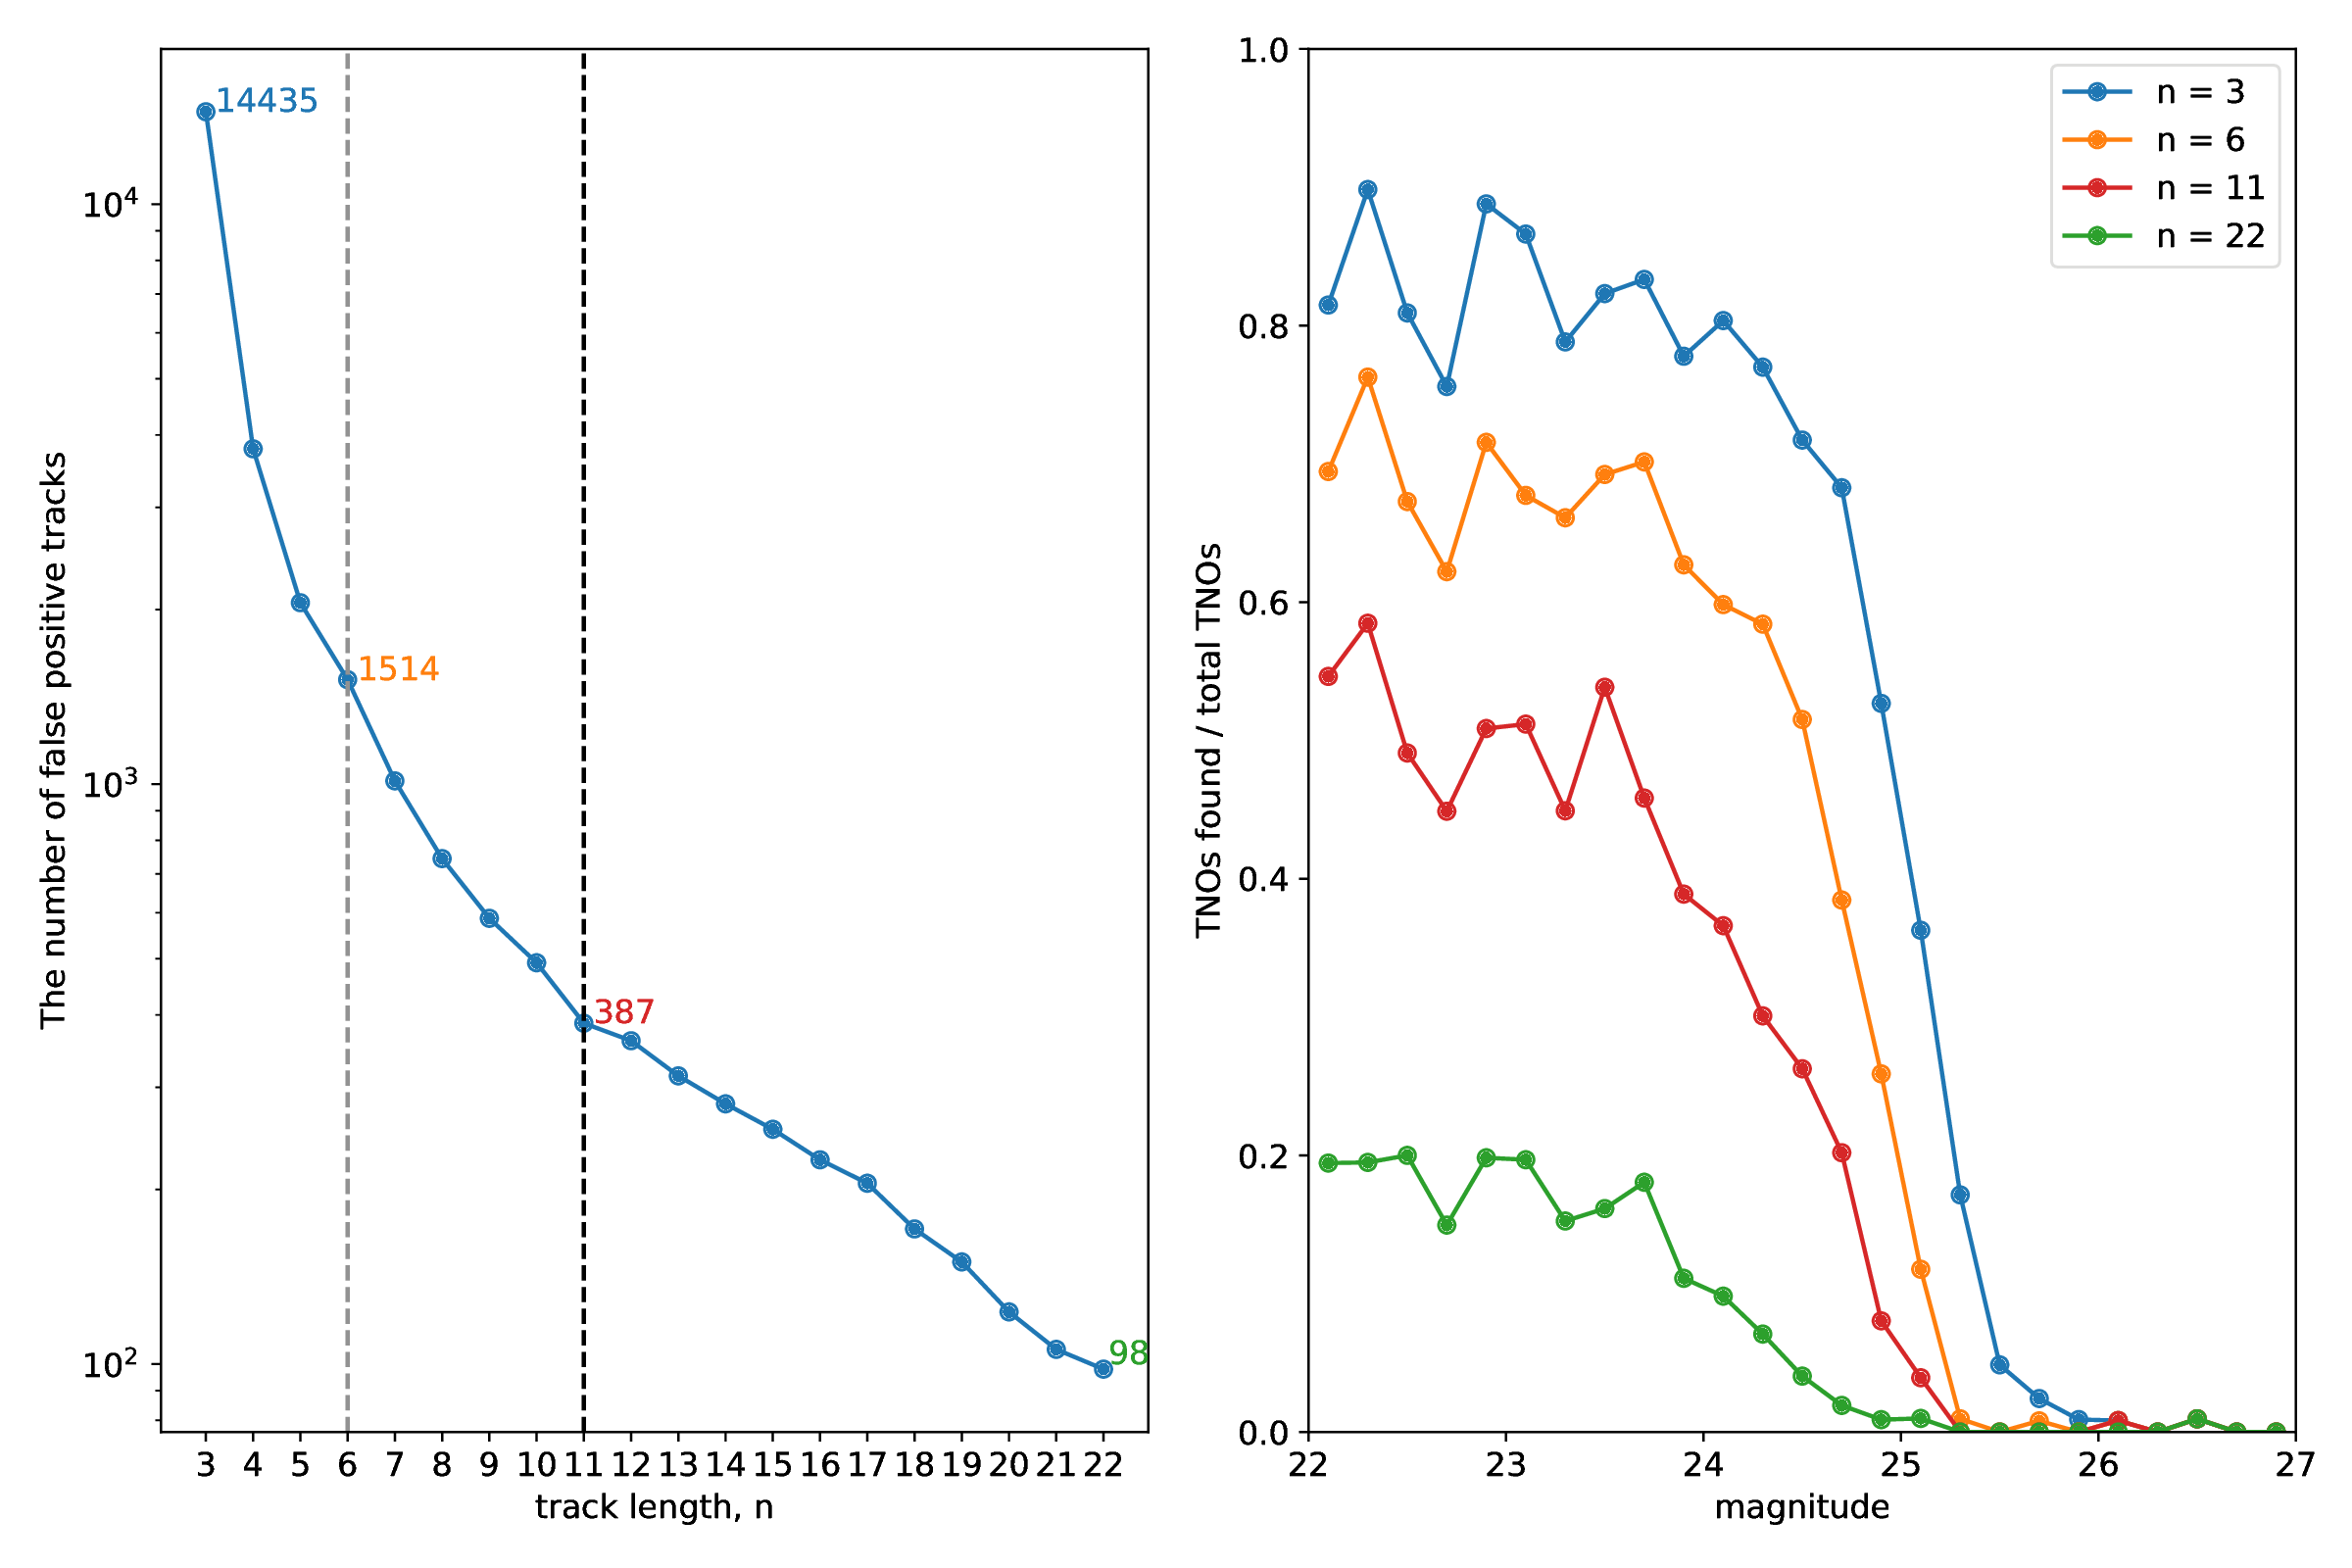
\includegraphics[width=\textwidth,keepaspectratio]{Figures/completeness_after_linear_fitting.png}
    \caption{Analysis of linear fitting approach on the C08132134 test set. (Left) Number of false positive tracks as a function of the minimum length of the track (n) to accept a track as a detection candidate.
    The vertical lines and end points are at n=3, n=6, n=11, and n=22.
    Setting the minimum track length requirement to these values would result in 14435, 1514, 387, and 98 candidates to vet respectively.
    (Right) A completeness graph showing artificial TNO retrieval rates as a function of magnitude for various track length.
    ``Found" objects did not go through the human inspection, therefore the actual retrieval rate will be slightly lower.
    Figure~\ref{fig:completeness single} is based on each single image pair classification result while the completeness shown here is for the final candidates after classification, and linear fitting.
    }
    \label{fig:completeness after Linear Fitting}
\end{figure}

%In this result section, we present how many planted TNOs this method found and missed on test sets C08, C13, C21, C34 with the effectiveness of Postprocessing processes.
%And then we present real SSOs we could be found on those sample test sets.

\subsection{Results with the Linear Fitting Approach}
\label{subsect:Retrieval rate on planted TNOs}

This subsection describes the results from the linear fitting approach.
Please refer to the section \ref{Subsect: Linear Fitting Approach} for the description of this approach.

The number of planted TNOs found strongly depended on the magnitude of objects.
On the whole, there were 2,910 planted sources added to C08, C13, C21, and C34.
In our final candidate list we retrieved 1,454 of these sources, with classification p$>$0.5 and track length n$>$3.
The ratio represents only a half success in retrieving planted sources in terms of the number of retrieved TNOs.
However, we detected a sharp decrease in detection ratio as the magnitude of TNOs increases.
If we divide the planted objects into magnitude bins and then analyze how many of them survived through the classification model and postprocessing algorithms, we observed that around 80\% of objects were detected when they were brighter than the 24th magnitude.
However, the detection rate dropped rapidly after the magnitude of 24.5 (Figure \ref{fig:completeness after Linear Fitting}, left side).
We can see that this method is quite effective at finding moving objects in astronomical images when the moving objects are sufficiently bright.
TNOs dimmer than the 25th magnitude were rarely retrieved as the SNR is low after the magnitude (refer Fig. \ref{fig:magexamples}). 
This behaviour is similar to the single image pair result shown on the Fig \ref{fig:completeness single}.

The longer the required track length, n, the more secure the detection but the fewer number of detection were made.
Without any postprocessing methods, the number of sub-image pairs is $\sim$960,000 at p$>$0.9 and $\sim$1,200,000 at p$>$0.5.
This would result in an impossible number of candidates for visual inspection.
The number of candidates diminishes quickly as we require n, the length of the tracks to be 3 or greater.
We marked that a track was correctly classified as a positive in this postprocessing algorithm when the actual position of a TNO was inside 3 pixels of the measured position of a TNO, and detection occurs more than or equal to n times.
With a requirement of a minimum length n=3, we retrieved 1,454 TNOs out of 2910 TNOs.
With a minimum requirement of a length n=6, we retrieved 1,220 TNOs.
With a minimum requirement of a length n=11, we retrieved 859 TNOs.
With a minimum requirement of a length n=22, we retrieved 240 TNOs (Figure \ref{fig:completeness after Linear Fitting}, right side).
The longer tracks enable confidence in the detection, but at a large cost of missing many potential TNOs.

To determine the right number of tracks to be inspected, we analyzed the relationship between the length of tracks and the number of tracks for false positive cases.
On the left side of the figure \ref{fig:completeness after Linear Fitting}, the number of tracks is very large with the minimum requirement of n=3.
However, the number decreases rapidly as we increase the minimum length.
For instance, With n=6, there were ten times fewer candidates compared to n=3.
We selected n=11 as the practical requirement for further inspection.
At that point, the number of false positives decreases to below 400 candidates, which translates to approximately 100 candidates per CCD.
Requiring n=22 does not yield good result at finding planted sources, even though inspecting candidates will be easier since the number of false positives per CCD is around 25.

% With those minimum length requirements, true positives yields are analyzed.
% The completeness curve on the right side of the figure \ref{fig:completeness after Linear Fitting} shows the ratio of detected TNOs compared to the total TNOs in each magnitude bin.
% n=3 is the minimum requirement we put to be a filtered detection, which means that the source could be linked with at least 2 other sources.
% n=6 is where the number of false positive candidates decreased significantly.
% We need to take a close look at n=11: often it is an artificial moving object, or sometimes it is a noise candidate from chip defects, bright background star.
% From n=11, each candidate becomes worthy enough to be inspected by humans because approximately 3/4 of tracks had a planted moving light source in them, with a feasible number of false positives.
% With the n=22 requirement, the yield on planted TNOs was very low, and was too weak to be used as a TNO detector even though the number of false positives was optimal.

With the n=11 minimum length requirement chosen, this method was effective to find artificial sources up to m=23.9 as it achieves approximately ``50\% retrieval rate" at the magnitude.
For our data set, it corresponds to SNR=7.2.
Note that the 50\% retrieval rate is not the absolute 50\%.
Because stars and galaxies block some parts of skies, some moving sources are intrinsically impossible to find (refer subsection \ref{subsect: Peak Detection Efficacy}).
This performance was not as good as we expected from utilizing a deep learning model, even before the visual inspection.

Upon inspecting false positive candidates manually with n=11 requirement or n=22 requirement, most of those tracks were definitely not non-planted SSOs, but rather caused by noises and wrong measurements on the positions.
Only very few of them included an SSO, and only one of them was a very slow object (approximately 3 arcseoncd/hour).

\subsection{High Precision Detection with the Probability Cumulative Approach}
\label{subsect: High precision with the Probability Cumulative Approach}

\begin{figure}[ht]
    \centering
    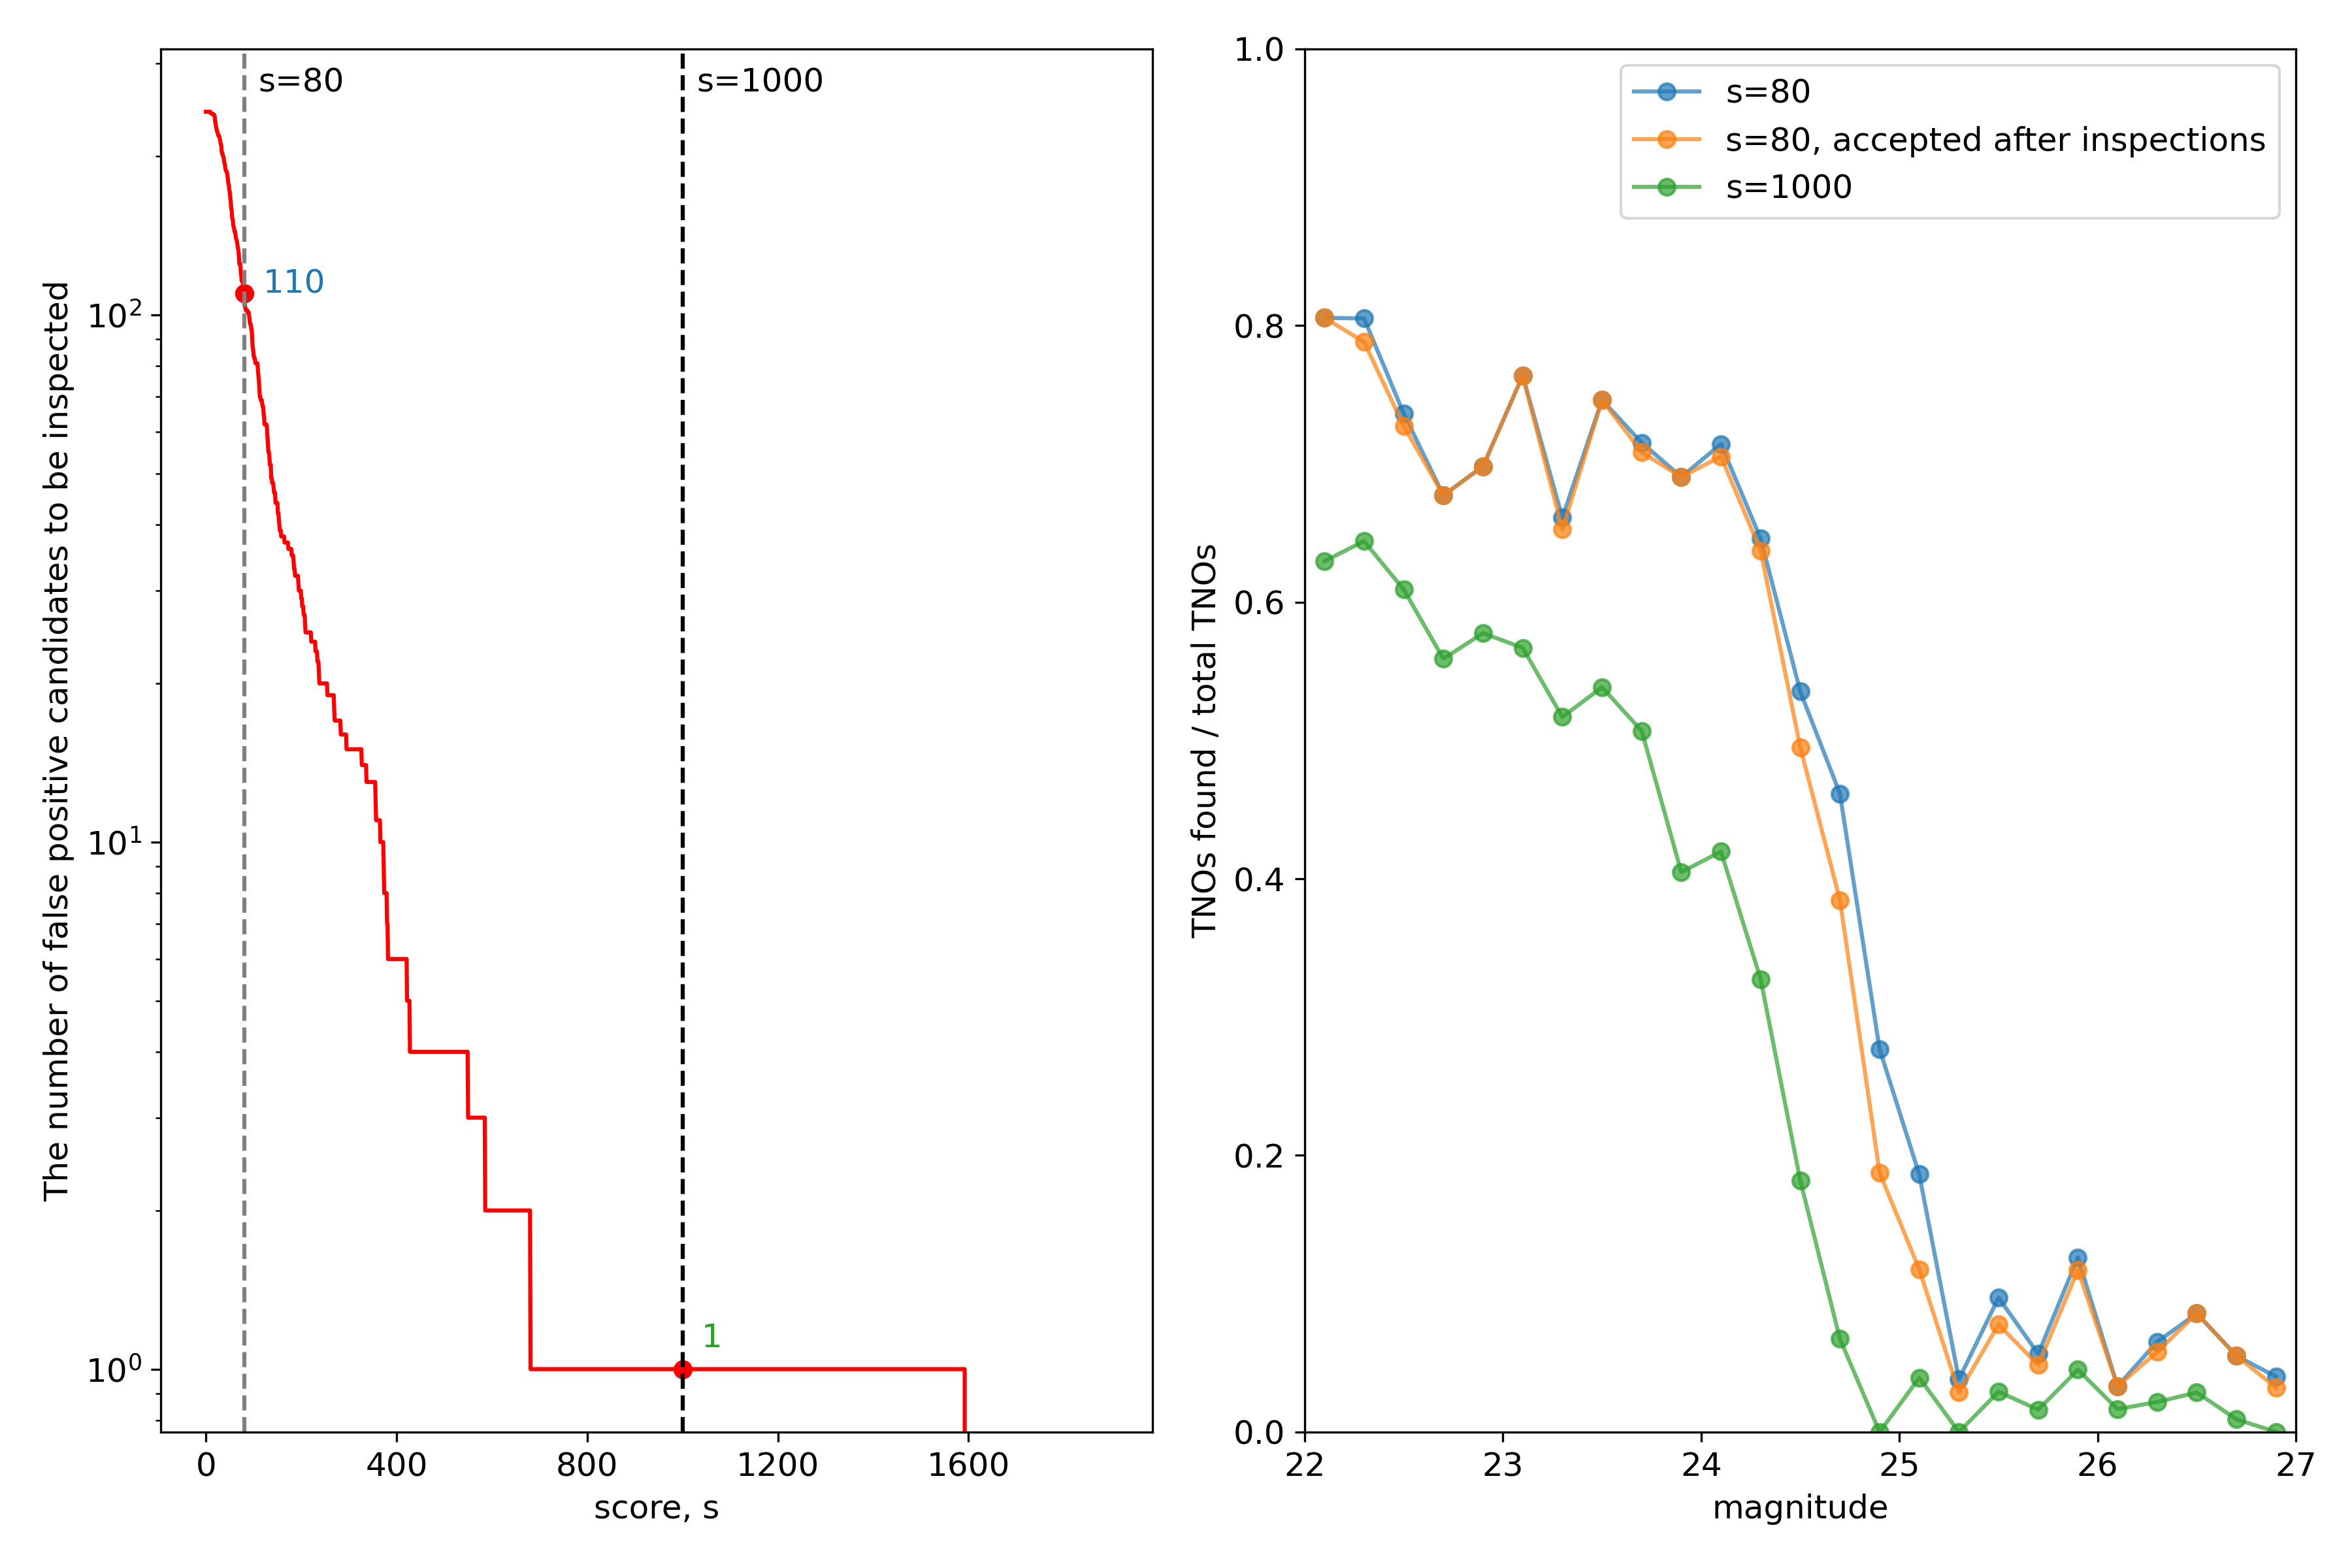
\includegraphics[width=\textwidth,keepaspectratio]{Figures/completeness_with_score.png}
    \caption{Analysis of scoring approach on the C08132134 test set (Left) Number of false positive sub-image series as a function of the minimum score of the sub-image series (n) to accept a sub-images series as a detection candidate.
    The vertical lines are at s=80 and s=1000.
    Setting the minimum score requirement to these values resulted in 110 and 1 false-positive candidates.
    (Right) A completeness graph showing artificial TNO retrieval rates as a function of magnitude for two kinds of score requirements and manual inspection requirement.
    Figure~\ref{fig:completeness single} is based on each single image pair classification result while this completeness graph is to show to the final number of TNOs found after postprocessing.
    }
    \label{fig:completeness with movies}
\end{figure}

Here we describe the results from the scoring approach.
Please refer to the section \ref{subsect: Scoring Approach} for the description of this approach.
For this approach, we marked that a sub-image series was correctly classified as a positive in this scoring approach when a moving object was in any sub-image of the series.

First of all, sub-image series with a very high score (s=1000 requirement) are confirmed to always have a moving object in them for our test set.
Out of 889 such sub-image series, 888 of them had an artificial TNO.
The only false positive in the set was a non-planted real slow-moving object (See Figure \ref{fig: a TNO with the largest probability}). 
From this result, candidates above a certain score can be indeed reported as slow SSOs without further inspection.
This capability of automatic detection can lead us to a total automation of SSO searches in future.

The large majority of sub-image series with a score of 80 or higher were found to be true positives.
Out of the 2085 sub-image series with high scores, 1975 were confirmed to contain an artificial TNO.
It means 95\% of GIFs produced with this method would have a moving source.
This high precision makes the manual inspection worth the time and effort and can be recommended as the final step of this discovery process.

The numbers of false positives were analyzed, and we find that this approach is effective at filtering on false positives while retaining true positives.
The number of false positives with the s=80 was 110 for the C08132134 data set, and this number 110 is similar to the 98 candidates given in the linear fitting approach with the length n=22 requirement, which was the most strict requirement (See the left side of the Figure \ref{fig:completeness after Linear Fitting}).
At the similar number of false positives, the number of successfully retrieved TNOs from the linear fitting approach was only 240, while the number of successfully retrieved TNOs from the scoring approach was 1390 for the s=80 requirement.
It is a significant improvement in the recall while keeping the number of false positive similar.

This method was effective at finding moving sources up to m=24.7.
For our data set, it corresponds to SNR=3.4, and is a performance comparable to the Outer Solar System Origin Survey \citep{2016AJ....152...70B}.
Note that OSSOS detection limit is based on searching a triplet of images, achieving a detection limit of about m=24.7 \citep{2018ApJS..236...18B}, whereas our search required three detections on 44 images.

There were several advantages of the scoring approach over the linear fitting approach.
This method excludes more false positives than the linear fitting approach.
Postprocessing steps were straightforward and took significantly less computing time.
The implementation of this method does not depend on the regression model, and hence we only need to train and use one model.
Furthermore, we can select the score threshold based on the research goal.
For example, bright and slow objects can be automatically claimed as an SSO without manual inspection.
Even when a moving object is dim, it is easier to spot the difference when the the moving object is shown in animations rather than inspecting each image separately.
Moving objects in a certain range of exposure duration appear sharp in our vision. \citep{1997Burr}
With these advantages, we achieved the high precision and high magnitude limit described above.

\subsection{Peak Detection Efficacy}
\label{subsect: Peak Detection Efficacy}

Even with the brightest TNOs in a data set, the recall does not reach 100\%.
For example, in the Figure \ref{fig:completeness single}, the recall is 80-90\% for the 22nd magnitude objects at the classification threshold of p=0.99.
The peak efficiency is determined by the level of crowding from stars and galaxies in the image.
Figure \ref{fig:obstacles} exhibits two common obstacles to source detection: bright sources and bad columns.
These types of obstacles hinder finding a moving object from the sub-images.
Therefore, even with the best detection process one does not anticipate detecting 100\% of the moving sources present in a series of images.

\begin{figure}[htb]
    \centering
    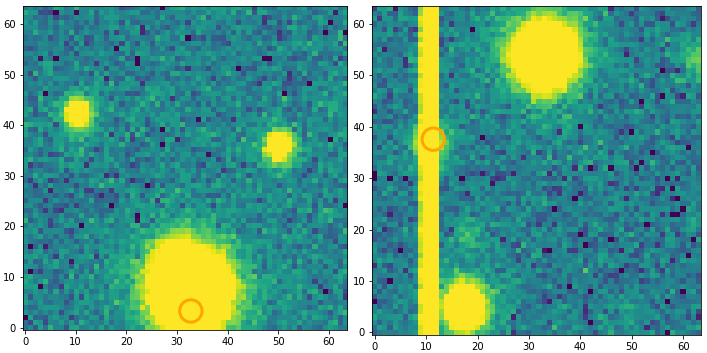
\includegraphics[width=0.5\textwidth,keepaspectratio]{Figures/obstacles.png}
    \caption{Sub-images containing artificial sources that were not detected by our process.
    The orange circles indicate the position at which the artificial source was added to the image.
    (Left) A bright stationary object (a star) in the background is obscuring the moving object.  
    (Right) Bad columns on the detector prevent the detection of the moving object.
    For these objects, the classification model assigns a low probability to the presence of a moving source.  
    For those that pass the classification step the regression model often fails to predict the correct position of the moving source and the candidate is rejected during the tracking process.
}
    \label{fig:obstacles}
\end{figure}

\subsection{Discovery of real SSOs}
\label{subsect:Discovery of real SSOs}

\begin{figure}
    \centering
    \includegraphics[width=0.9\textwidth,keepaspectratio]{Figures/a_TNO_with_the_largest_probability.png}
    \caption{A sub-image series accepted as being a detected solar system object.
    The images in the grid are arranged in rows and columns, at the same sky coordinates, depicting the progression of time.
    The time interval between each image is 248 seconds.
    The images are arranged in a sequential order from left to right, and from top to bottom.
    This non-planted candidate returned the highest score from our method.
    Pixel scale is 0.185 arcsecond per pixel.
    Based on the rate of motion of $\sim$3 arcsecond per hour, this object is likely to be a Centaur or a TNO.
    }
    \label{fig: a TNO with the largest probability}
\end{figure}

\begin{figure}
    \centering
    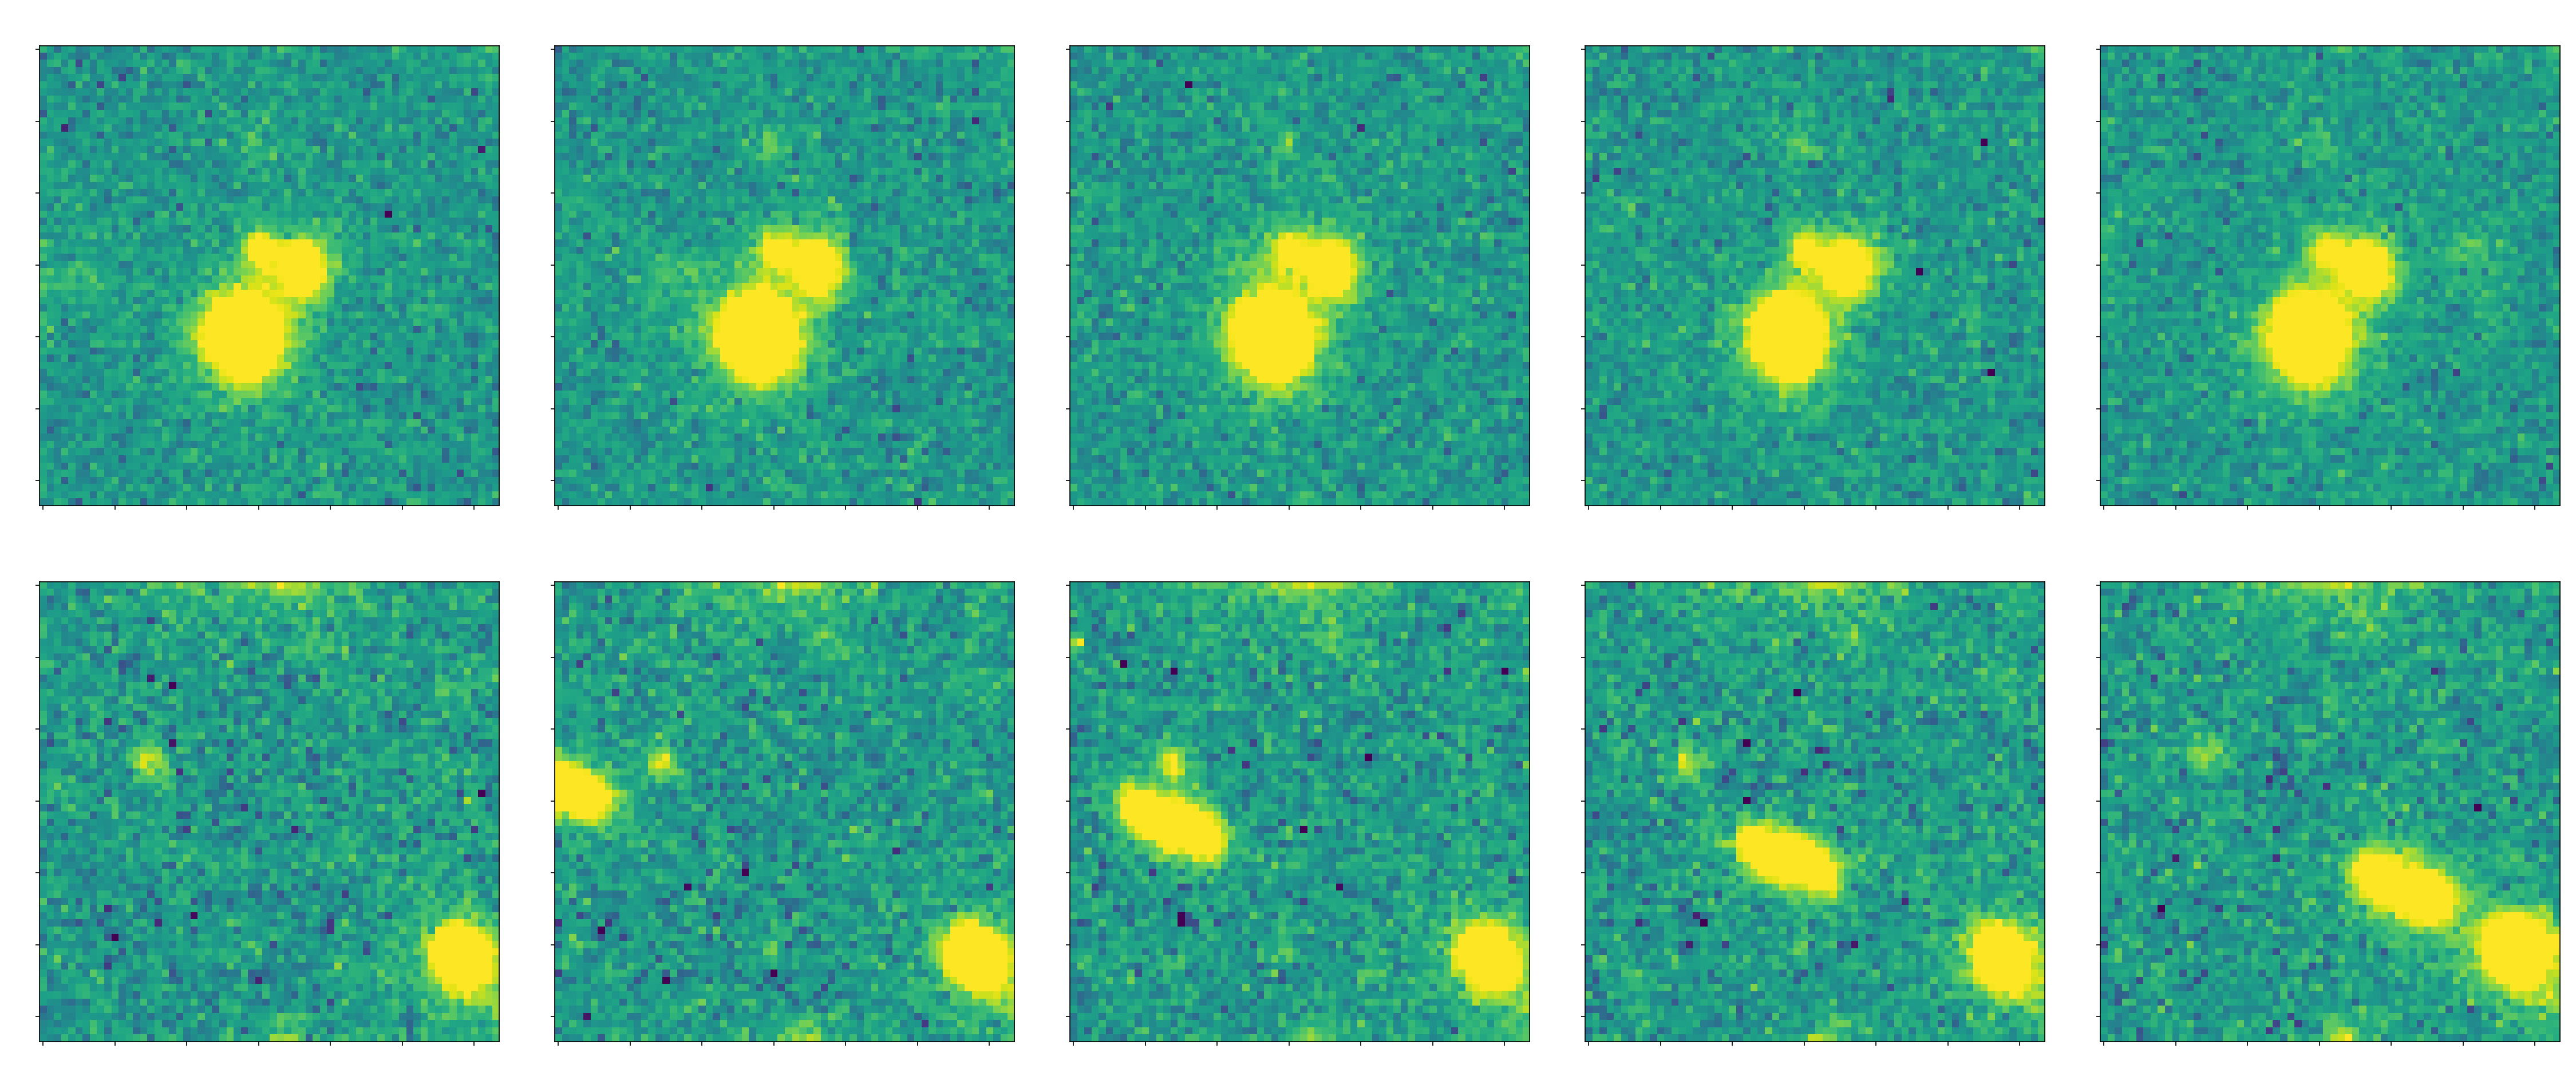
\includegraphics[width=0.9\textwidth,keepaspectratio]{Figures/SSO_examples.png}
    \caption{Sub-image series examples accepted as being detected SSOs.
    The images are arranged in sequential order from left to right.
    The first row: A dim oval-shaped light source moves from the center-left to the center-right almost horizontally.
    The moving object is easier to spot when images are made into an animation.
    The second row: A bright oval-shaped light source moves from the center-left to the lower right.
    Based on their rate of motion, these objects are likely to be asteroids.
    }
    \label{fig: SSO examples}
\end{figure}

The visual inspection with the scoring approach was done for non-planted areas of our data sets to examine its capability to find real SSOs.
Out of 835 highly scored sub-image series (s$\geq$80), 424 sub-image series had a non-planted SSO that we could visibly and confidently confirm.
Some of them appeared more than once in another sub-image series as they move across the sky, and the 424 sub-image series containing a moving source included 196 unique SSOs.
The candidates that passed this visual inspection may then be confirmed by follow-up observations.

The majority of discovered objects had sky motion in excess of 15 arcseconds per hour, but a handful of slow moving objects, which could be TNOs were also found.
Note that the low number of discoveries on slow objects is not because the method is more sensitive to finding fast objects; it is rather because asteroids in a particular magnitude range outnumber TNOs: The method was actually more sensitive to smaller and slower objects because they spent more time in the sub-image frame and resulted in very high scores.
One of the slow-moving objects is shown on Figure~\ref{fig: a TNO with the largest probability}.
We also report examples of fast-moving objects on Figure~\ref{fig: SSO examples}.

The initial intention of this study was to find TNOs with deep learning techniques, but after postprocessing steps we found that this method could also find other SSOs such as asteroids.
The model was trained using image pairs that have small time (minimum of 4 minutes) and large time (maximum of 3 hours) offsets between the images.
This enabled the model to be sensitive to objects with fast rates of motion (sources well offset between two sub-images with a small time offset) and slower rates of motion (sources well offset between two sub-images with a large time offset).
The fast non-planted moving sources also exhibited trailing, indicating that the final model was not particularly sensitive to the shape of the PSF used in creating the artificial sources.

\section{Summary and Conclusion}
This study applied CNN-based networks to detect SSOs in CFHT MegaCam/MegaPrime images.
For our test data set, we used a series of 44 exposures (each approximately 205 seconds) that had been acquired as part of a search for satellites of Saturn in July 2019.
Artificial moving sources were added to the original images and used to train a variety of network architectures.
Of the architectures examined, we found that CNNs and particularly ImageNet algorithms were particularly adept at classifying images as containing or not containing a moving source.
There were 7 architectures compiled: the FCNN for comparison, the modified AlexNet, the modified VGG, ResNet50, ResNet50V2, MobileNet and MobileNetV2.
Out of those, we determined that ResNet50V2 and MobileNet have the best performance for our study.
We selected MobileNet for moving source detection because it has fewer parameters, making it lightweight.

We also found that MobileNet is more effective when trained using examples from multiple CCDs rather than a single CCD.
Models constructed by training on a single CCD were ineffective at finding moving sources on other CCDs.
This may be due to the training having latched onto the image shape, or some other characteristic specific to the CCD and the artificial source addition process, rather than object motion.

The sub-images pairs were further accessed by postprocessing steps such as the linear fitting approach or the scoring approach.
The linear fitting approach was an approach to group nearby moving object positions measured by the trained regression model, and remove outliers to build postprocessed candidates.
The linear fitting approach was not very effective at retrieving planted TNOs without significant visual inspection.
Alternatively, a scoring approach was developed to return a likelihood (score) of having a moving object in a sub-image series at a fixed sky position.
When a score from a sub-image series was significantly high, exceeding 1000, the sub-image series could be claimed as an automatic detection without further manual inspection; otherwise, if the score was relatively high, exceeding 80, the sub-image series was subjected to manual inspection for the presence of a moving source.
The manual inspection was worth the time as 95\% of the sub-image series classified as positives were true positives.
The approach diminished the number of candidates substantially and effectively retrieved planted TNOs as low as SNR=3.6, and it was sensitive to SSO over a broad range of motion rates.
Passing the image pairs into the classifier and analyzing scores, we discovered planted and non-planted SSOs in an automated manner.

Using this approach we have demonstrated that the two-channel MobileNet architecture can be effectively trained to enable the detection of moving sources in astronomical images.
Using the process above resulted in the detection of slow and fast-moving solar system objects, even though the model was only trained using slow-moving sources.
The future study can involve adapting this method to other data sets, and exploring other deep learning techniques to improve the results.

\section{Acknowledgements}

Based on observations obtained with MegaPrime/MegaCam, a joint project of CFHT and CEA/DAPNIA, at the Canada-France-Hawaii Telescope (CFHT) which is operated by the National Research Council (NRC) of Canada, the Institut National des Science de l'Univers of the Centre National de la Recherche Scientifique (CNRS) of France, and the University of Hawaii. The observations at the Canada-France-Hawaii Telescope were performed with care and respect from the summit of Maunakea which is a significant cultural and historic site.

This research used the Canadian Advanced Network For Astronomy Research (CANFAR) operated in partnership by the Canadian Astronomy Data Centre and The Digital Research Alliance of Canada with support from the National Research Council of Canada the Canadian Space Agency, CANARIE and the Canadian Foundation for Innovation.

\clearpage

% \begin{figure}
%     \centering
%     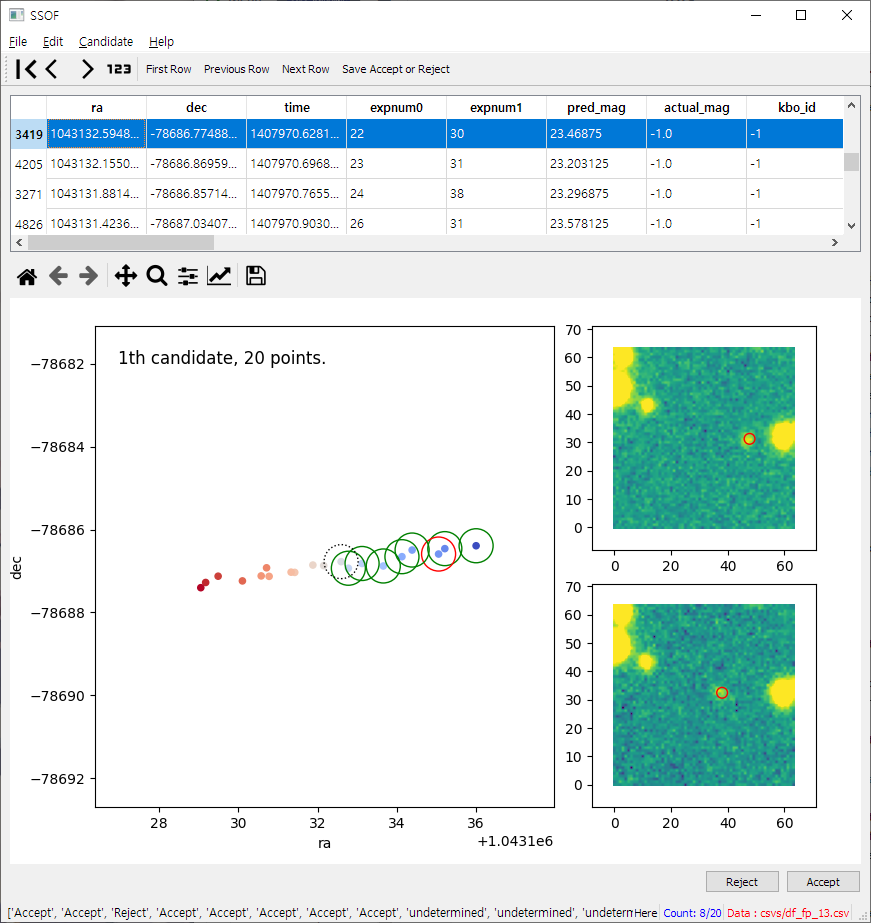
\includegraphics[width=0.8\textwidth,keepaspectratio]{SSOF_05.png}
%     \caption{SSOF is an application to vet the final candidates derived from ML classification and tracking process. On the top, the table containing information such as predicted positions/magnitudes, time of observation is presented. On the left, a scatter plot showing all sources connected together are shown on the sky coordinate system. On the right, a pair of sub-images are drawn.}
%     \label{fig:Visual Inspection}
% \end{figure}

% \begin{figure}
%     \centering
%     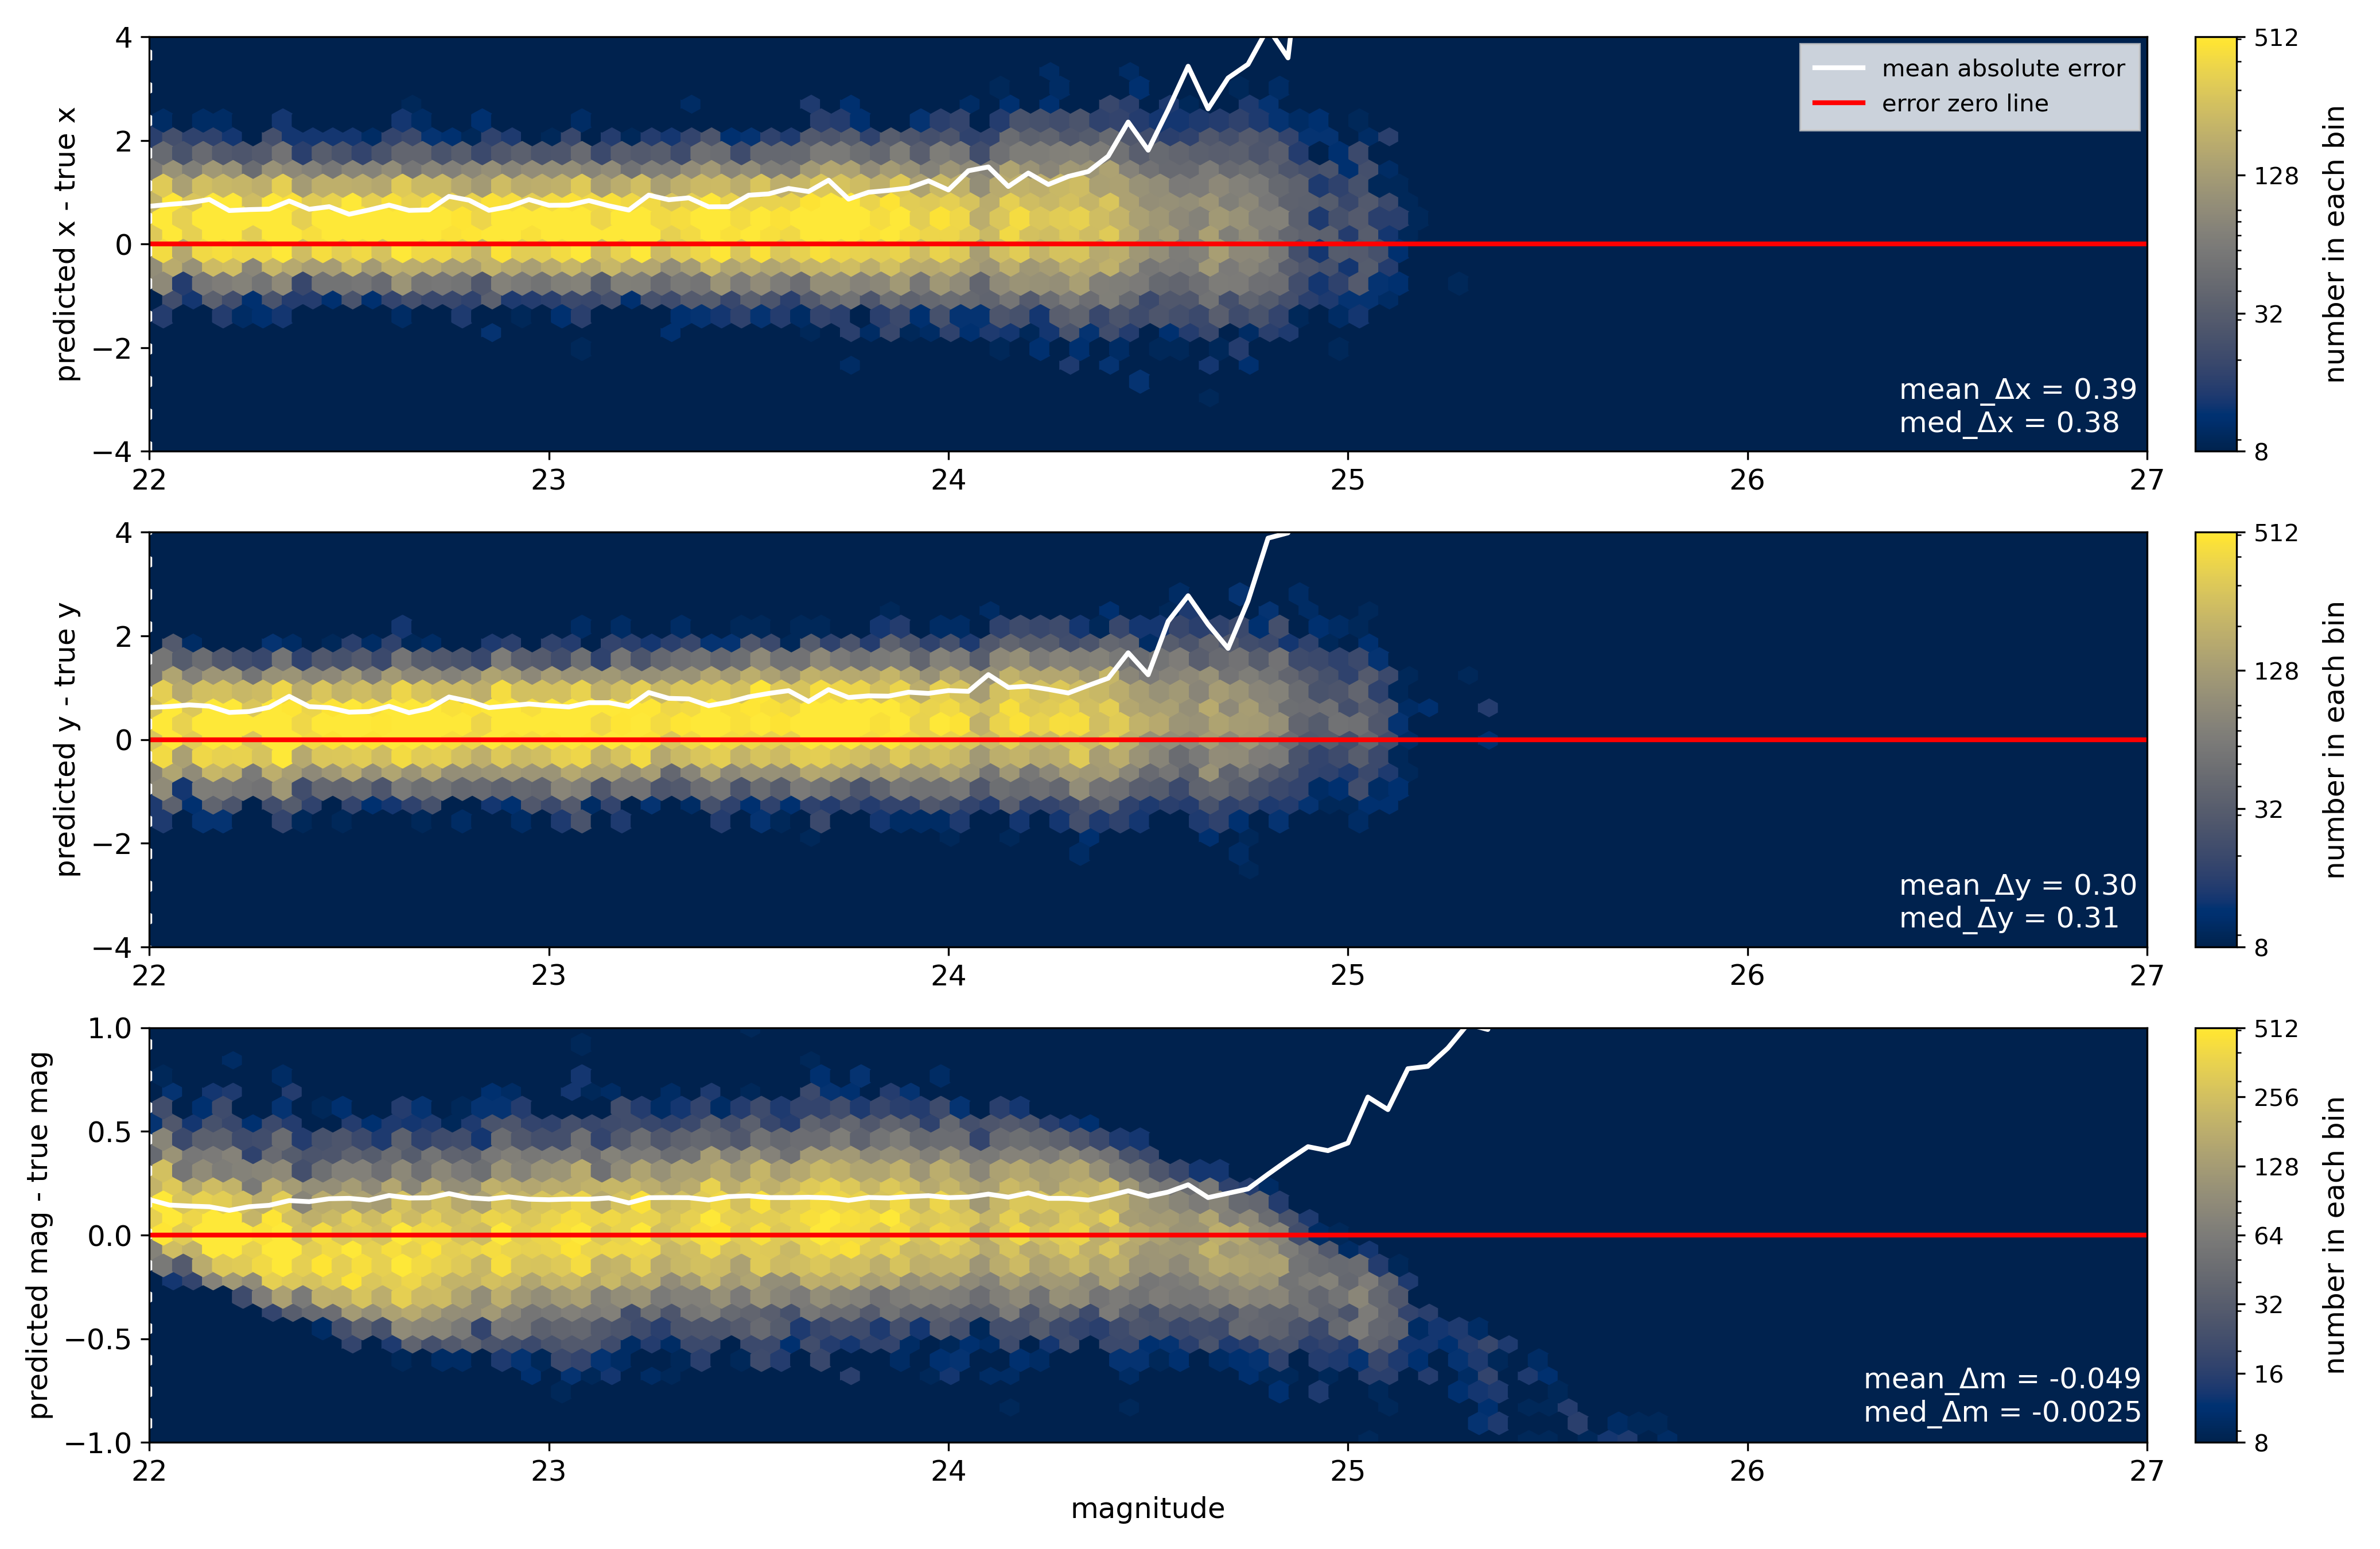
\includegraphics[width=\textwidth,keepaspectratio]{mag_vs_error_hexbin.png}
%     \caption{Hexagonal binning plot to show the performance of regression model trained, which predicts the position of TNOs, compared to the magnitude of TNOs. Upper: magnitude up to 23. centre: magnitude up to 25. Lower: magnitude up to 27.}
%     \label{fig:rgs_magnitude}
% \end{figure}

% \begin{figure}
%     \centering
%     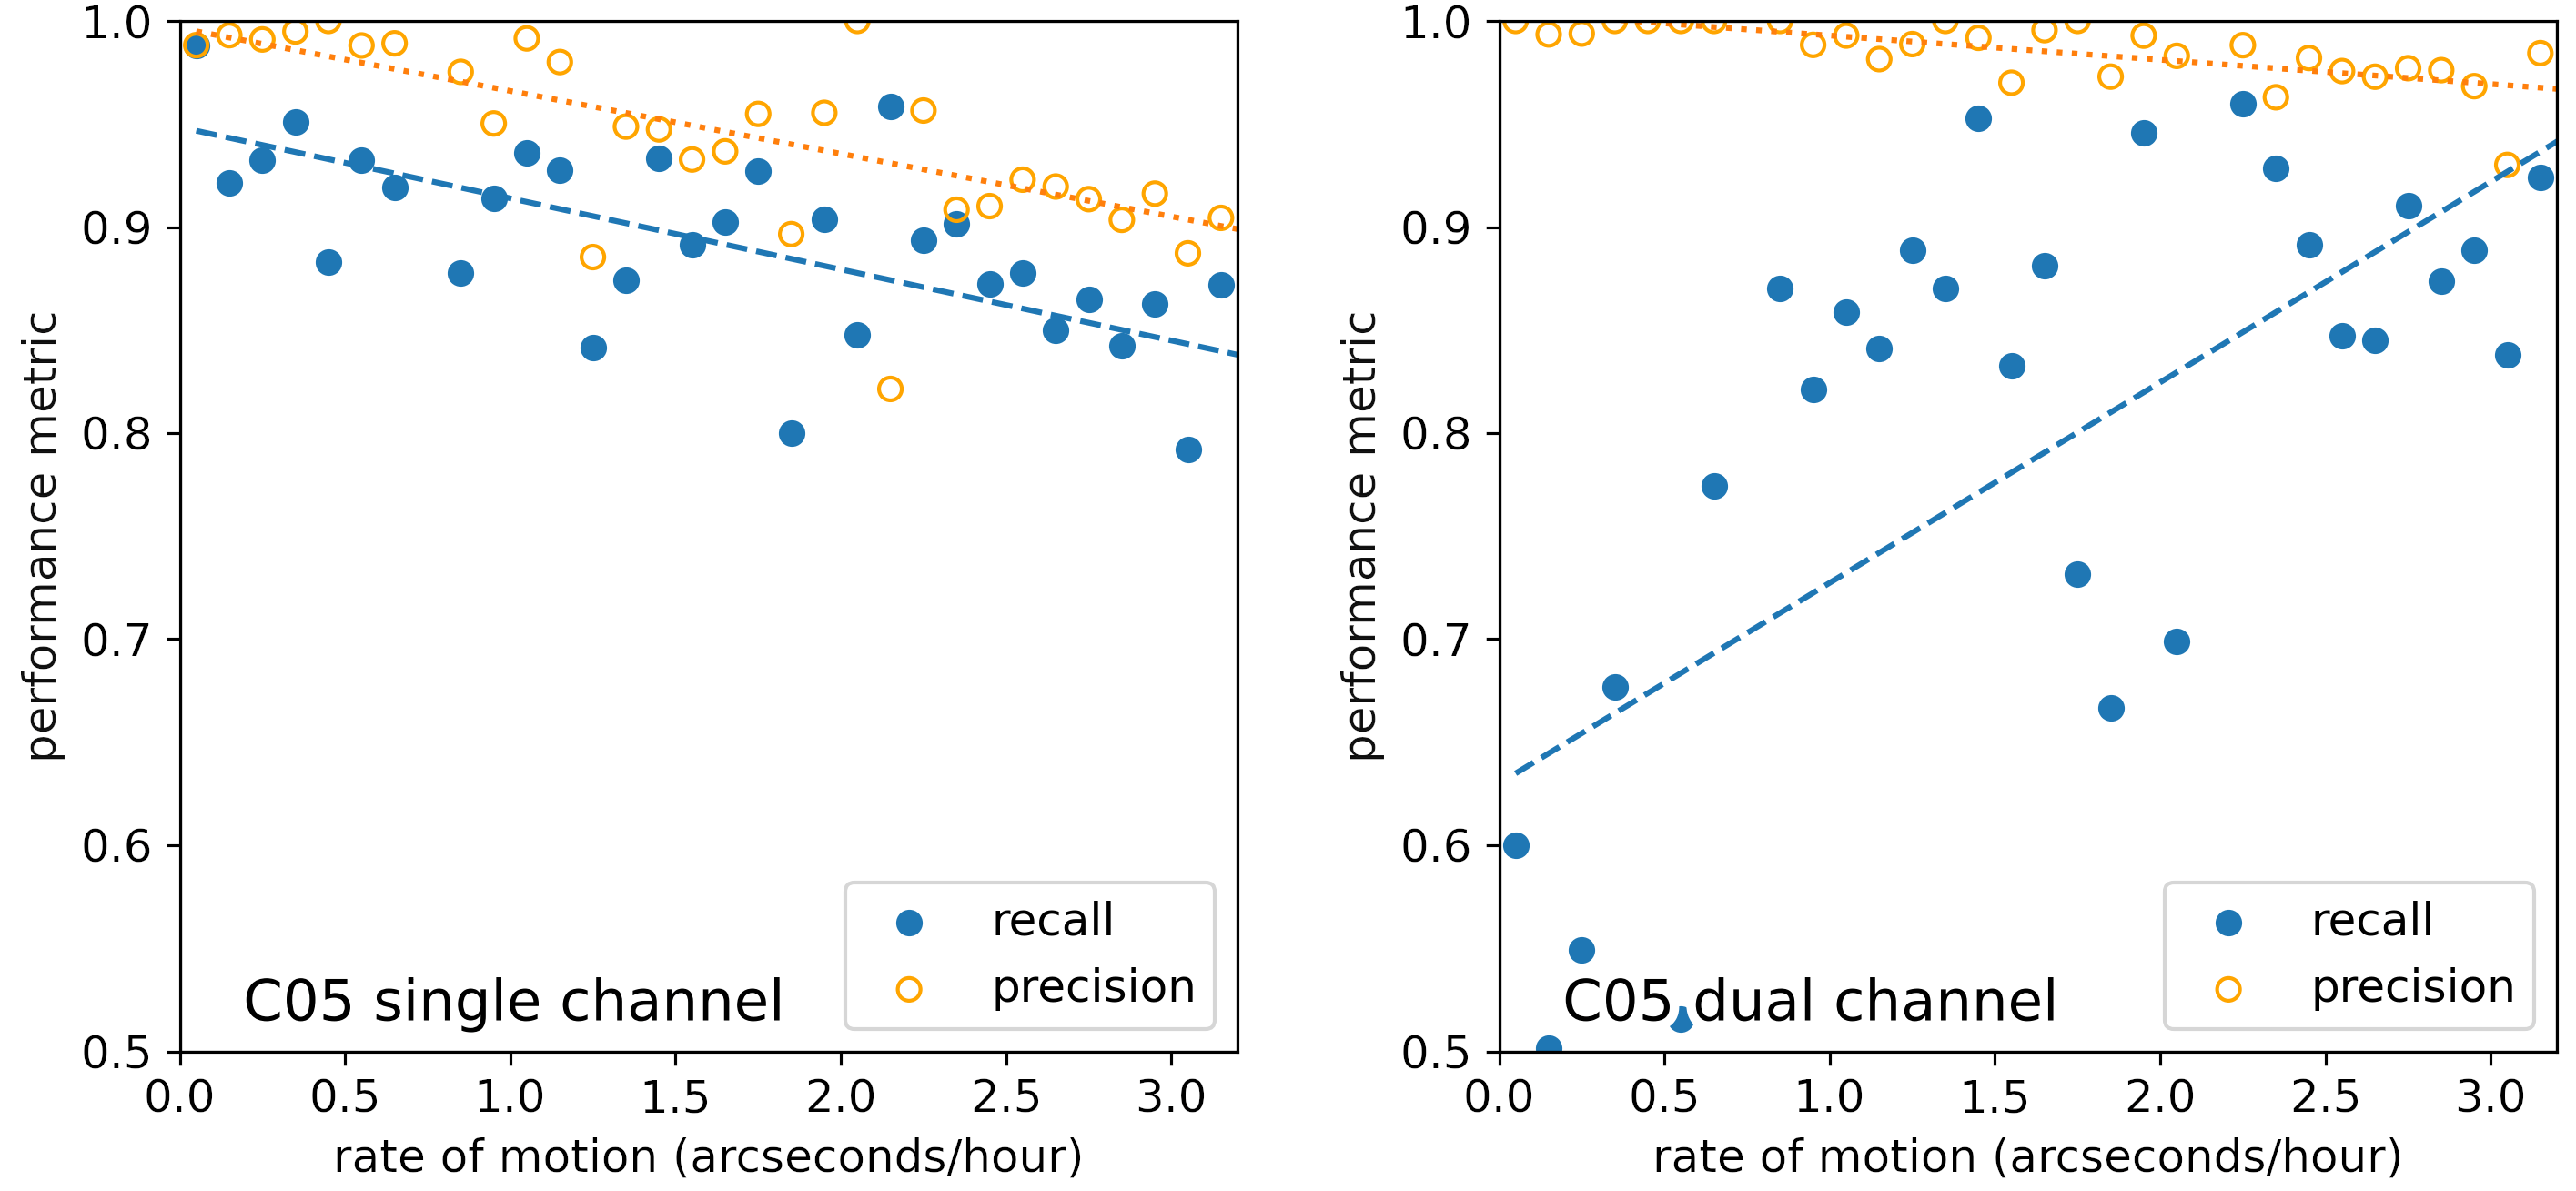
\includegraphics[width=0.75\textwidth,keepaspectratio]{singledual.png}
%     \caption{Scatter plots of rate of motion of TNOs and classifier performance metrics are shown. Recall and precision are explained at Equation \ref{eq:rpf}. These plots show that the single channel data sets and double channel data sets train the models in different ways. Each dot had a bin with 0.1"/hour and the metrics were calculated separately. Regarding the number of cutouts in the bins, Approximately 15\% of cutouts with a TNO had rates of motion smaller than 2"/hour, and only approximately 5\% of cutouts with a TNO had rates of motion larger than 3"/hour. Therefore a majority of TNOs in positive cutouts had rates of motion between 2"/hour and 3"/hour. The performance metrics of the single channel training (left plot) are clearly decreasing as the rate of motion increases. However, the recall of the dual channel training (right plot) is significantly increasing as the rate of motion increases while the precision is sufficiently high for all rates of motion.}
%     \label{fig:rate_vs_agreement}
% \end{figure}


\clearpage

\bibliography{TNODiscoverer}
\end{document}